\PassOptionsToPackage{unicode=true}{hyperref} % options for packages loaded elsewhere
\PassOptionsToPackage{hyphens}{url}
\PassOptionsToPackage{dvipsnames,svgnames*,x11names*}{xcolor}
%
\documentclass[man,floatsintext]{apa6}
\usepackage{lmodern}
\usepackage{amssymb,amsmath}
\usepackage{ifxetex,ifluatex}
\usepackage{fixltx2e} % provides \textsubscript
\ifnum 0\ifxetex 1\fi\ifluatex 1\fi=0 % if pdftex
  \usepackage[T1]{fontenc}
  \usepackage[utf8]{inputenc}
  \usepackage{textcomp} % provides euro and other symbols
\else % if luatex or xelatex
  \usepackage{unicode-math}
  \defaultfontfeatures{Ligatures=TeX,Scale=MatchLowercase}
\fi
% use upquote if available, for straight quotes in verbatim environments
\IfFileExists{upquote.sty}{\usepackage{upquote}}{}
% use microtype if available
\IfFileExists{microtype.sty}{%
\usepackage[]{microtype}
\UseMicrotypeSet[protrusion]{basicmath} % disable protrusion for tt fonts
}{}
\IfFileExists{parskip.sty}{%
\usepackage{parskip}
}{% else
\setlength{\parindent}{0pt}
\setlength{\parskip}{6pt plus 2pt minus 1pt}
}
\usepackage{xcolor}
\usepackage{hyperref}
\hypersetup{
            pdftitle={Transfer of Learned Opponent Models in Zero Sum Games},
            pdfauthor={Ismail Guennouni~\& Maarten Speekenbrink},
            colorlinks=true,
            linkcolor=blue,
            filecolor=Maroon,
            citecolor=Blue,
            urlcolor=Blue,
            breaklinks=true}
\urlstyle{same}  % don't use monospace font for urls
\usepackage{graphicx,grffile}
\makeatletter
\def\maxwidth{\ifdim\Gin@nat@width>\linewidth\linewidth\else\Gin@nat@width\fi}
\def\maxheight{\ifdim\Gin@nat@height>\textheight\textheight\else\Gin@nat@height\fi}
\makeatother
% Scale images if necessary, so that they will not overflow the page
% margins by default, and it is still possible to overwrite the defaults
% using explicit options in \includegraphics[width, height, ...]{}
\setkeys{Gin}{width=\maxwidth,height=\maxheight,keepaspectratio}
\setlength{\emergencystretch}{3em}  % prevent overfull lines
\providecommand{\tightlist}{%
  \setlength{\itemsep}{0pt}\setlength{\parskip}{0pt}}
\setcounter{secnumdepth}{0}
% Redefines (sub)paragraphs to behave more like sections
\ifx\paragraph\undefined\else
\let\oldparagraph\paragraph
\renewcommand{\paragraph}[1]{\oldparagraph{#1}\mbox{}}
\fi
\ifx\subparagraph\undefined\else
\let\oldsubparagraph\subparagraph
\renewcommand{\subparagraph}[1]{\oldsubparagraph{#1}\mbox{}}
\fi

% set default figure placement to htbp
\makeatletter
\def\fps@figure{htbp}
\makeatother

\shorttitle{Upgrade Report}
\affiliation{
\vspace{0.5cm}
\textsuperscript{1} Department of Experimental Psychology, University College London}
\usepackage{csquotes}
\usepackage{upgreek}
\captionsetup{font=singlespacing,justification=justified}

\usepackage{longtable}
\usepackage{lscape}
\usepackage{multirow}
\usepackage{tabularx}
\usepackage[flushleft]{threeparttable}
\usepackage{threeparttablex}

\newenvironment{lltable}{\begin{landscape}\begin{center}\begin{ThreePartTable}}{\end{ThreePartTable}\end{center}\end{landscape}}

\makeatletter
\newcommand\LastLTentrywidth{1em}
\newlength\longtablewidth
\setlength{\longtablewidth}{1in}
\newcommand{\getlongtablewidth}{\begingroup \ifcsname LT@\roman{LT@tables}\endcsname \global\longtablewidth=0pt \renewcommand{\LT@entry}[2]{\global\advance\longtablewidth by ##2\relax\gdef\LastLTentrywidth{##2}}\@nameuse{LT@\roman{LT@tables}} \fi \endgroup}
\shorttitle{}
\thispagestyle{headings}
\title{Transfer of Learned Opponent Models in Zero Sum Games}
\author{Ismail Guennouni\textsuperscript{1}~\& Maarten Speekenbrink\textsuperscript{1}}
\date{}

\authornote{

Correspondence concerning this article should be addressed to Ismail Guennouni, Department of Experimental Psychology, University College London, 26 Bedford Way, London WC1H 0AP, United Kingdom. E-mail: \href{mailto:i.guennouni.17@ucl.ac.uk}{\nolinkurl{i.guennouni.17@ucl.ac.uk}}}

\abstract{
Human learning transfer abilities take advantage of important cognitive building blocks such as an abstract representation of concepts underlying tasks and
causal models of the environment. One way to build abstract representations of the environment when the task involves interactions with others is to build
a model of the opponent that may inform what actions they are likely to take next. In this study, we propose to explore opponent modelling and its transfer with the use of
computer agents possessing human-like theory of mind abilities with limited degrees of iterated reasoning. Through two differentiated experiments, we find that participants can
deviate from Nash equilibrium play and learn to adapt to the opponent strategy and exploit it. Moreover, we showed that participants transfer their learning to new games and that
the transfer is moderated by the level of sophistication of the opponent. Computational modelling shows that it is likely that players start each game using a model-based
learning strategy that facilitates generalisation and opponent model transfer, but then switch to behaviour that is consistent with a model-free learning strategy in the latter
stages of the interaction.


}

\begin{document}
\maketitle

\hypertarget{introduction}{%
\section{Introduction}\label{introduction}}

Being able to transfer previously acquired knowledge to a new domain is one of the hallmarks of human intelligence. Humans are naturally endowed with the ability to extract relevant features from a situation, identify the presence of these features in a novel setting and use previously acquired knowledge to adapt to previously unseen challenges using acquired knowledge. More formally, Perkins \& Salomon (1992) define transfer of learning as the application of skills, knowledge, and/or attitudes that were learned in one situation to another learning situation. This typically human skill has so far eluded modern AI agents. Deep neural networks for instance can do very well on image recognition tasks and can even reach super-human performance levels on video and strategic board games. Yet they struggle to learn as fast or as efficiently as humans do, and more importantly they have a very limited ability to generalize and transfer knowledge to new domains. Lake, Ullman, Tenenbaum, \& Gershman (2017) argue that human learning transfer abilities take advantage of important cognitive building blocks such as an abstract representation of concepts underlying tasks and compositionally structured causal models of the environment.

One way to build abstract representations of the environment when the task involves interactions with others is to build a model of the person we are interacting with that may inform what actions they are likely to take next. Once we learn something about them, we can use this knowledge to inform how to best behave in novel situations. This may lead to very efficient generalization of knowledge, even to situations that are dissimilar to the history of interaction, assuming what we have learned about others is an abstract representation that is not too dependent on the environment of the initial interaction. There is evidence that people learn models of their opponents when they play repeated economic games (Stahl \& Wilson, 1995), engage in bilateral negotiations (Baarslag, Hendrikx, Hindriks, \& Jonker, 2016), or simply try to exploit a non random player in chance games such as Rock-Paper-Scissors (Weerd, Verbrugge, \& Verheij, 2012). In this paper, we are specifically interested in the way in which people build and use models of their opponent to facilitate learning transfer, when engaged in situations involving an interaction with strategic considerations. These situations arise frequently such as in negotiations, auctions, strategic planning and all other domains in which theory of mind (Premack \& Woodruff, 1978) abilities play a role in determining human behaviour. In order to explore learning transfer in these strategic settings, it is generally useful to study simple games as a model of more complex interactions. More specifically, we need a framework that allows the study of whether and how a player takes into consideration, over time, the impact of its current and future actions on the future actions of the opponent and the future cumulative rewards. Repeated games, in which players interact repeatedly with the same opponent and have the ability to learn about the opponent's strategies and preferences (Mertens, 1990) are particularly adapted to the task of opponent modelling.

In exploring opponent modelling and learning transfer, most studies adopted two types of opponents in the experimental setting. Either human participants were matched with other participants or they played against a computer algorithm. Computer opponents were generally programmed not to change their strategies over the course of the task, allowing better experimental control. One of the commonalities in studies of how humans adapt to computerised opponents is that they have mostly looked at the ability of players to detect and exploit action-based learning rules. The strategies implemented by the computer opponents had a style of play that was not \enquote{human-like} in the sense that humans are not very good at playing specific mixed strategies with any precision, or at detecting patterns from long sequences of past play due to cognitive constraints. It is therefore important to have agents that \enquote{play like humans}, and one way of achieving that is to embed theses agents with human-like theory of mind abilities. Simon (1972) explains that humans have limited cognitive capacities and as such cannot be expected to solve computationally complex problems such as finding Nash equilibria. Instead, they will try to \enquote{satisfice} by choosing a strategy that is adequate in a simplified model of the environment, rather than an optimal one. This concept finds its natural application in \enquote{level-k} theory, first adopted by Stahl \& Wilson (1995). It posits that deviations from Nash equilibrium solutions in simple games are explained by the fact that humans have a heterogeneous degree of strategic sophistication. At the bottom of the ladder, level-0 players are non-strategic and play either randomly or use a salient strategy in the game environment Arad \& Rubinstein (2012). Level-1 players are next up the ladder of strategic sophistication and will assume all their opponents belong to the level-0 category and as such will best respond to them given this assumption. Likewise, a level-2 player will choose actions that are the best response given the belief that all opponents are exactly one level below, and so on.

In this study, we propose to explore opponent modelling and its transfer with the use of computer agents possessing human-like theory of mind abilities with limited degrees of iterated reasoning. The agents will either be a level-1 or level-2 player, mimicking human theory of mind abilities and the limited recursion depth they exhibit (Goodie, Doshi, \& Young, 2012). Our choice of using computer opponents instead of matching groups of participants makes it easier to disentangle the process of learning about the opponent from that of learning about the game structure and payoffs. When playing against other human opponents, players are learning about the game as well as trying to infer the potential dynamic strategy of the opponent simultaneously. Thus, it is harder to focus on an individual and how her strategies are changing and adapting to the opponent's play if we cannot experimentally control the behaviour of the opponent. The use of computer opponents to elicit learning behavior has been explored in the literature with encouraging results. For instance, Spiliopoulos (2013) made humans play constant sum games against 3 computer opponents, designed to take advantage of known patterns in human play such as imperfect randomization and heuristics use. He found that human participants do adapt to the opponent they are facing. Shachat \& Swarthout (2004) made human participants face computer opponents playing various mixed strategies in a zero-sum asymmetric matching pennies game. They found that the players changed their strategies towards exploiting the deviations of the opponent from the Mixed Strategy Nash Equilibrium (MSNE), and that this exploitation was very likely if the deviation from the MSNE play was high.
We measure transfer of learning about the opponent strategy between games with varying degrees of similarity. The first two games we use are structurally identical except for action labels. In one experiment, the third game is strategically similar to the first two but descriptively different, while in a second experiment, we introduce a third game that is dissimilar to the first two in terms of payoff matrix and strategic structure. In the first experiment, participants face the same opponent throughout the three games, and the opponents are randomised to be either level-1 or level-2 players. In the second experiment, participants faced both level-1 and level-2 opponent sequentially, with the order in which they are faced randomised across participants.

\newpage

\hypertarget{experiment-1}{%
\section{Experiment 1}\label{experiment-1}}

\hypertarget{methods}{%
\subsection{Methods}\label{methods}}

\hypertarget{participants-and-design}{%
\subsubsection{Participants and Design}\label{participants-and-design}}

A total of 52 (28 female, 24 male) participants were recruited on the Prolific Academic platform. The mean age of participants was 31.2 years. Participants were paid a fixed fee of £2.5 plus a bonus dependent on their performance which averaged £1.06. The study used a 2 (computer opponent: level 1 or level 2) by 3 (games: rock-paper-scissors, fire-water-grass, numbers) design, with repeated measures on the second factor.

\hypertarget{tasks}{%
\subsubsection{Tasks}\label{tasks}}

In the first experiment, the three games were rock-paper-scissors, fire-water-grass and the numbers game. A typical rock-paper-scissors game (hereafter RPS) is a 3x3 zero sum game, with a cyclical hierarchy between possible actions: rock blunts scissors, paper wraps rock, and scissors cut paper. If one player chooses an action which dominates their opponent's action, the player wins (receives a reward of 1) and the other player loses (receives a reward of -1). Otherwise it is a draw and both players receive a reward of 0. It has a unique MSNE consisting of randomly playing one of the three options each time. The second game is identical to Rock-Paper-Scissors in all but action labels. We call it Fire-Water-Grass (FWG): Fire burns grass, water extinguishes fire, and grass absorbs water. We are interested in exploring whether learning is transferred in a fundamentally similar game where the only difference is in the description of the choice actions. Finally, the numbers game is a generalization of rock-paper-scissors. In the variant we use, 2 participants concurrently pick a number between 1 and 5. To win in this game, a participant needs to pick a number exactly 1 higher than the number chosen by the opponent. For example, if a participant thinks their opponent will pick 3, they ought to choose 4 to win the round. To make the strategies cyclical as in RPS, the game stipulates that the lowest number (1) beats the highest number (5), so if the participant thinks the opponent will play 5, then the winning choice is to pick 1. This game has a structure similar to RPS in which every action is dominated by exactly one choice. All other possible combination of choices that are not consecutive are considered ties. A win would add 1 point to the score of the player, while a loss deduces one point and a tie does not affect the score. Similar to RPS, the MSNE is to play each action with equal probability in a random way.

\hypertarget{procedure}{%
\subsubsection{Procedure}\label{procedure}}

Participants played 3 games sequentially against the same computer opponent. The computer opponent either used a level-1 or level-2 strategy. Participants were informed they would play three different games against the same computer opponent. Each participant plays all three games consecutively and in the same order described above. Participants were told that the opponent cannot cheat and will choose its actions simultaneously without knowledge of the participant's choice. A total of 50 rounds of each game was played with the player's score displayed at the end of each game. The score was calculated as the number of wins minus the number of losses. Ties did not affect the score. In order to incentivise the participants to maximise the number of wins against the opponents, players were paid a bonus at the end of the experiment that was proportional to their final score. Each point is worth £0.02. An example of the interface for the rock-paper-scissors game is provided in Figure~\ref{fig:feedback-rps-exp2}.

\begin{figure}

{\centering 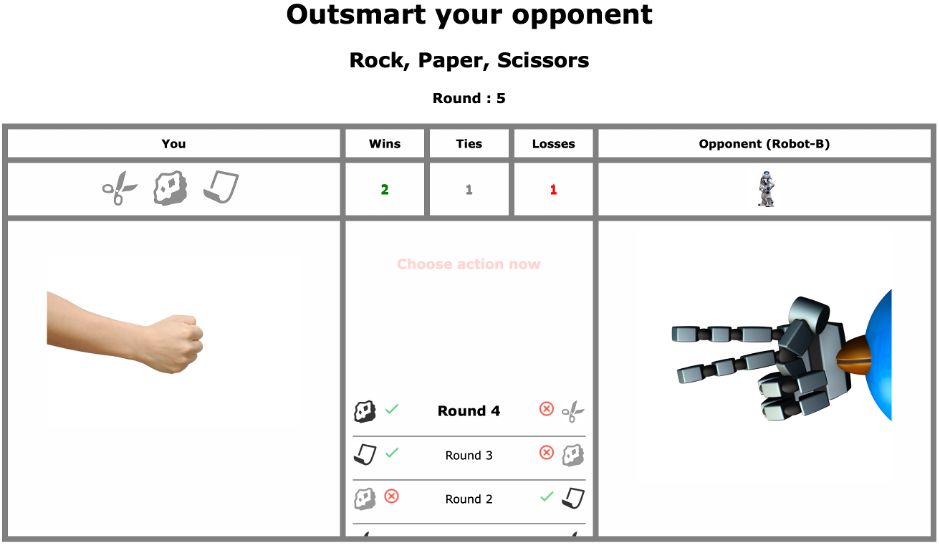
\includegraphics{images/feedback_rps} 

}

\caption{Screenshot of the feedback at the end of a round of Rock-Paper-Scissors}\label{fig:feedback-rps-exp2}
\end{figure}

\hypertarget{results}{%
\subsubsection{Results}\label{results}}

\begin{figure}

{\centering 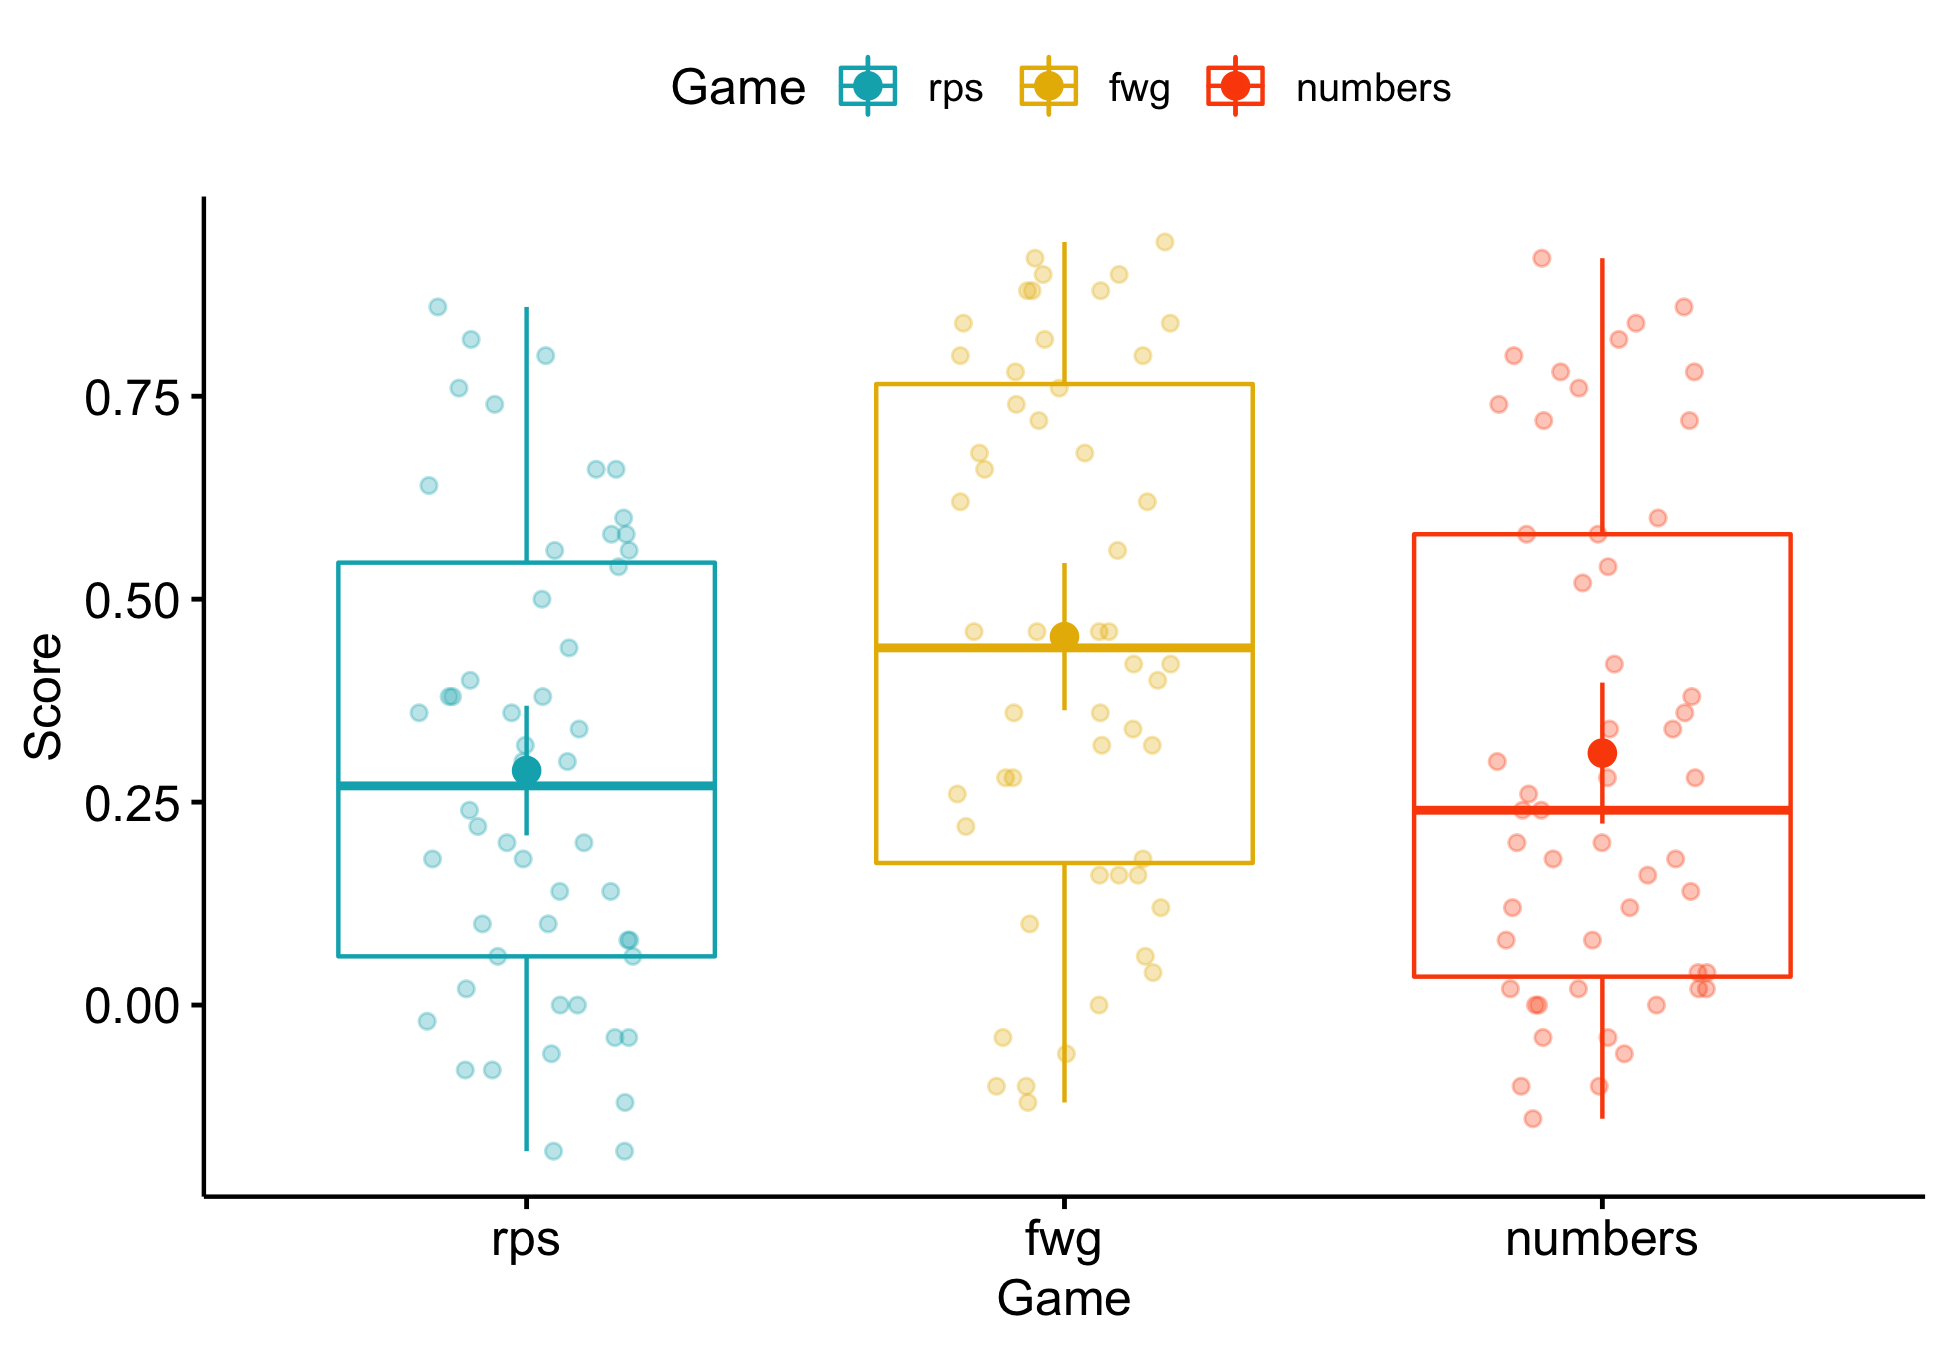
\includegraphics{draft_upgrade_v1_files/figure-latex/exp1-avg-scores-game-1} 

}

\caption{Boxplot of scores per game across conditions}\label{fig:exp1-avg-scores-game}
\end{figure}

Looking at the aggregate scores (See Figure~\ref{fig:exp1-avg-scores-game} ), the RPS game had the lowest average score across participants (M = 0.289, SD = 0.348) followed by NUMBERS (M = 0.31, SD = 0.347) and finally the FWG game had the highest average score (M = 0.454, SD = 0.354). Aggregate average scores for each game were significantly different from 0 (hypothesised value of random play) using parametric one sample t-tests (RPS: t(51) = 7.26, \(p\) \textless{} 0.001 ; FWG: t(51) = 10.04 , \(p\) \textless{} 0.001 ; NUMBERS: t(51) = 7.17, \(p\) \textless{} 0.001).
To analyse within and between game learning, we used a 2 (condition: level-1, level-2) by 3 (game: RPS, FWG, NUMBERS) by 2 (block: first half, second half) repeated measures ANOVA with the first factor varying between participants. There was a main effect of Game (F(2,100) = 8.54, \(\eta^{2}\) = 0.05, p \textless{} 0.001), showing that average scores varied significantly over the games. Post-hoc pairwise comparisons showed that performance in the FWG game was significantly higher than in the RPS game (t(100) =3.78, p = 0.0008), and the performance in the NUMBERS game was significantly lower than FWG game (t(100) = -3.32 , p = 0.0024). The score in RPS was not significantly different from the score in NUMBERS (t(100) = 0.45 , p = 0.65). The main effect of Block (F(1,50) = 22.51 , p \textless{} .001, \(\eta^{2}\) = 0.03) shows that the average score in the first half of games (M = 0.29) was significantly lower than in the second half of the games played (M = 0.40), which translates to within-game learning. The main effect of Condition (F(1,50) = 5.44, p = .024, \(\eta^{2}\) = 0.05) indicates that scores were higher against the level-1 player (M = 0.43) than against the level-2 player (M = 0.27). This indicates that it was harder for participants, on average, to exploit the strategy of the more sophisticated opponent (level-2) compared to that of the comparatively less sophisticated agent (level-1).

\begin{figure}

{\centering 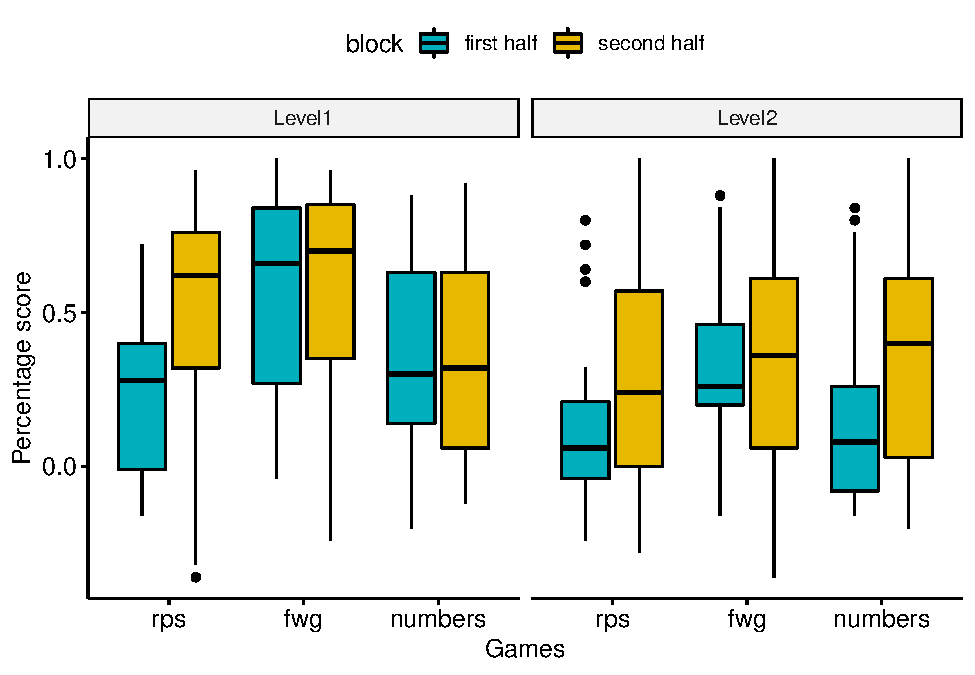
\includegraphics{draft_upgrade_v1_files/figure-latex/exp1-3factor-plot-1} 

}

\caption{Boxplots of scores by game, block and condition}\label{fig:exp1-3factor-plot}
\end{figure}

Finally, the analysis showed a significant block by game interaction ( F(2,100) = 6.92 , p = .002, \(\eta^{2}\) = 0.02), indicating that within-game learning differed between the games. Indeed, second half scores in RPS are significantly higher than first-half scores (t(150) = 5.59, p \textless{}.0001), while there was no significant difference between block scores for the other two games. This is indicative of the significant within-game learning happening in the first game when players have no experience against the opponent, as opposed to much lower within game performance improvement in the latter games when participants have had some experience playing against the opponent and start with higher scores indicative of transfer. There was also a three-way interaction between condition, game, and block ( F(2,100) = 3.88, p = .023, \(\eta^{2}\) = 0.01), which indicates, as seen in Figure~\ref{fig:exp1-3factor-plot} that within-game learning changes across games also depend on the sophistication of the opponent. For instance, there is more within game learning in the third game against level-2 opponents, since the initial scores are lower than against level-1 opponent. The explanation for this will become clearer when we discuss the factors moderating learning transfer in the next section.

\hypertarget{learning-transfer}{%
\subsubsection{Learning transfer}\label{learning-transfer}}

As a measure for learning transfer, we focus on participants' scores in the first 5 rounds excluding the initial round (rounds 2-6). We exclude the very first round as the computer opponent plays randomly here and there is no opportunity yet for the human player to exploit their opponent's strategy. A group of players with no experience of the game are expected to perform at chance level over the early rounds of a new game, as was the case in RPS. Positive scores in the early rounds would therefore reflect generalization of prior experience. For the FWG game, the score is significantly higher than 0 ( t(148.85) = 4.58 , p \textless{} 0.0001). This is also the case for the more dissimilar game : NUMBERS ( t(148.85) = 3.00, p = 0.0092). For the RPS game, the average score is not significantly different from 0 as this is the first game and no learning is possible (t(148.85) = 1.04 , p = 0.89).



\begin{figure}

{\centering 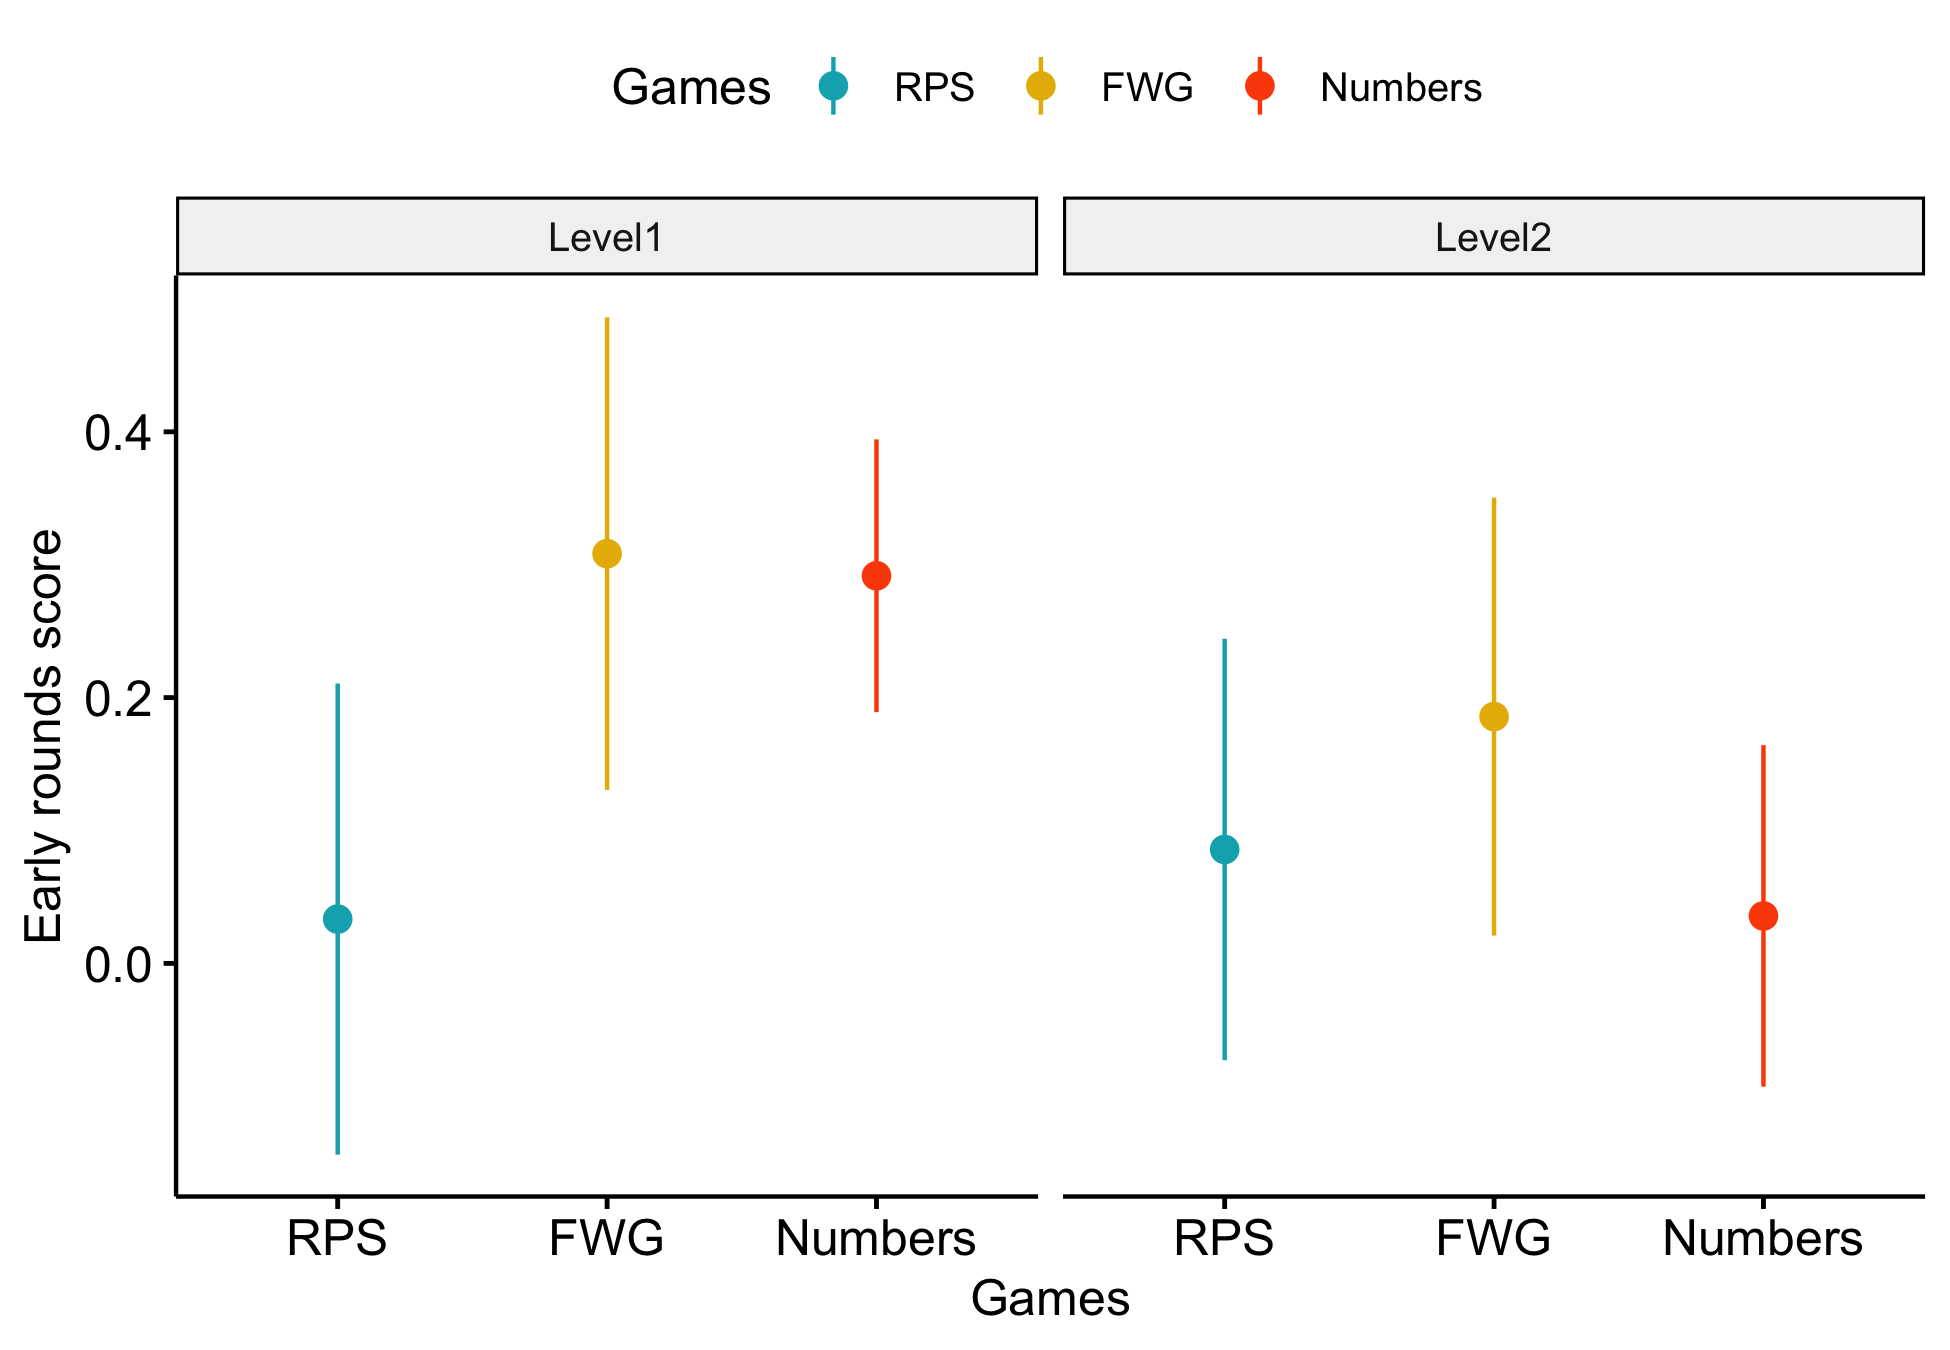
\includegraphics{draft_upgrade_v1_files/figure-latex/exp1-score-by-opp-1} 

}

\caption{Mean and 95\% confidence Intervals of early scores by game and opponent}\label{fig:exp1-score-by-opp}
\end{figure}

Next, we explore whether learning transfer is moderated by the type of opponent and game similarity. Figure~\ref{fig:exp1-score-by-opp} shows the mean scores for rounds 2-6 by game for both level-1 and level-2 facing players as well as the \(95\) percent confidence interval for the mean. Graphically we can see that the pattern is dissimilar between level-1 and level-2 players, and we suspect transfer to be positively associated with similarity and negatively with degree of sophistication of the agent. To explore this, we run statistical tests on early round scores by game and opponent against the null hypothesis of 0 (no transfer). For level-1 facing players, there is evidence of learning transfer from RPS to both FWG ( t(150) = 3.96, p \textless{} 0.001) and NUMBERS (t(150) = 3.74, p \textless{} 0.001) . For level-2 facing players, there is evidence for transfer from RPS to the similar game FWG, albeit scores are lower than for level-1 player ( t(150) = 2.48, p = 0.01) but not to the dissimilar game of NUMBERS.

\hypertarget{discussion-experiment-1}{%
\subsubsection{Discussion Experiment 1}\label{discussion-experiment-1}}

Our results when averaging across conditions (previous section) showed that there was indeed evidence for transfer to the more dissimilar game (NUMBERS). We can see from splitting the participants by opponent faced that this transfer is exclusively driven by level-1 facing players, as average early round scores of level-2 facing players are close to nil in the NUMBERS game. Therefore, both participants facing level-1 and level-2 agents can transfer learning to the similar game, but only those facing the less sophisticated opponent are able to generalise to the less similar game.

\hypertarget{experiment-2}{%
\section{Experiment 2}\label{experiment-2}}

We ran a second experiment with various differentiated features to improve the opportunity to measure learning transfer. Instead of making participants face either the level-1 or level-2 player throughout, we made them face both opponents sequentially. Because there were two distinct opponents, requiring potentially holding two opponent models in memory, we also made it easier to recall the results of past rounds by providing participants with the opportunity to see the history of the game since the beginning of each interaction. Figure~\ref{fig:feedback-rps-exp2} shows an example of showing interaction history in the RPS game. Finally, we changed the third game to a penalty shootout game, which has the same number of actions as the first two. If we see evidence for differential play against opponents, it would show participants adapting their strategies to the opponent they are facing, which is indicative of opponent modelling.

\hypertarget{methods-1}{%
\subsection{Methods}\label{methods-1}}

\hypertarget{participants-design}{%
\subsubsection{Participants \& Design}\label{participants-design}}

A total of 48 participants (21 females, 28 males, 1 unknown) used the Prolific Academic platform to participate in the experiment. This was a new set of participants unrelated to those taking part in Experiment 1. The average age of players was 30.2 years, and the mean duration to complete the task was 39 minutes. Participants were incentivised using a two-tier payment mechanism: a fixed fee of £2.5 for completing the experiment plus a performance linked bonus that averaged £1.32.

\hypertarget{tasks-1}{%
\subsubsection{Tasks}\label{tasks-1}}

The three games the participants played were Rock-Paper-Scissors, Fire-Water-Grass, and the penalty shootout game. The first two games were identical to the ones used in the first experiment. In the final game (shootout) the participants took the role of the player shooting a football (soccer) penalty, with the AI opponent being the goalkeeper. Players had the choice between three actions, like in the first two games: Shooting the football to the left, right or centre of the goal. If the player shoots in a direction different from that of where the goalkeeper dives, they win the round and the goalkeeper loses. Otherwise, the goalkeeper catches the ball and the player loses the round. There is no possibility of ties in this game. Figure~\ref{fig:screenshot-shootout} shows a snapshot of play in the shootout game. What makes this game different however is that there are two ways to beat the opponent in each round: if we think the opponent is going to choose \enquote{'right}' in the next round, we can win by both choosing \enquote{'left}' and \enquote{'center}'. A level-1 player (thinks that his opponent will repeat his last action) has two ways to win the next round. As such, we have programmed the level-2 computer program to choose randomly between the two possibilities that a level-1 player may choose.

\begin{figure}

{\centering 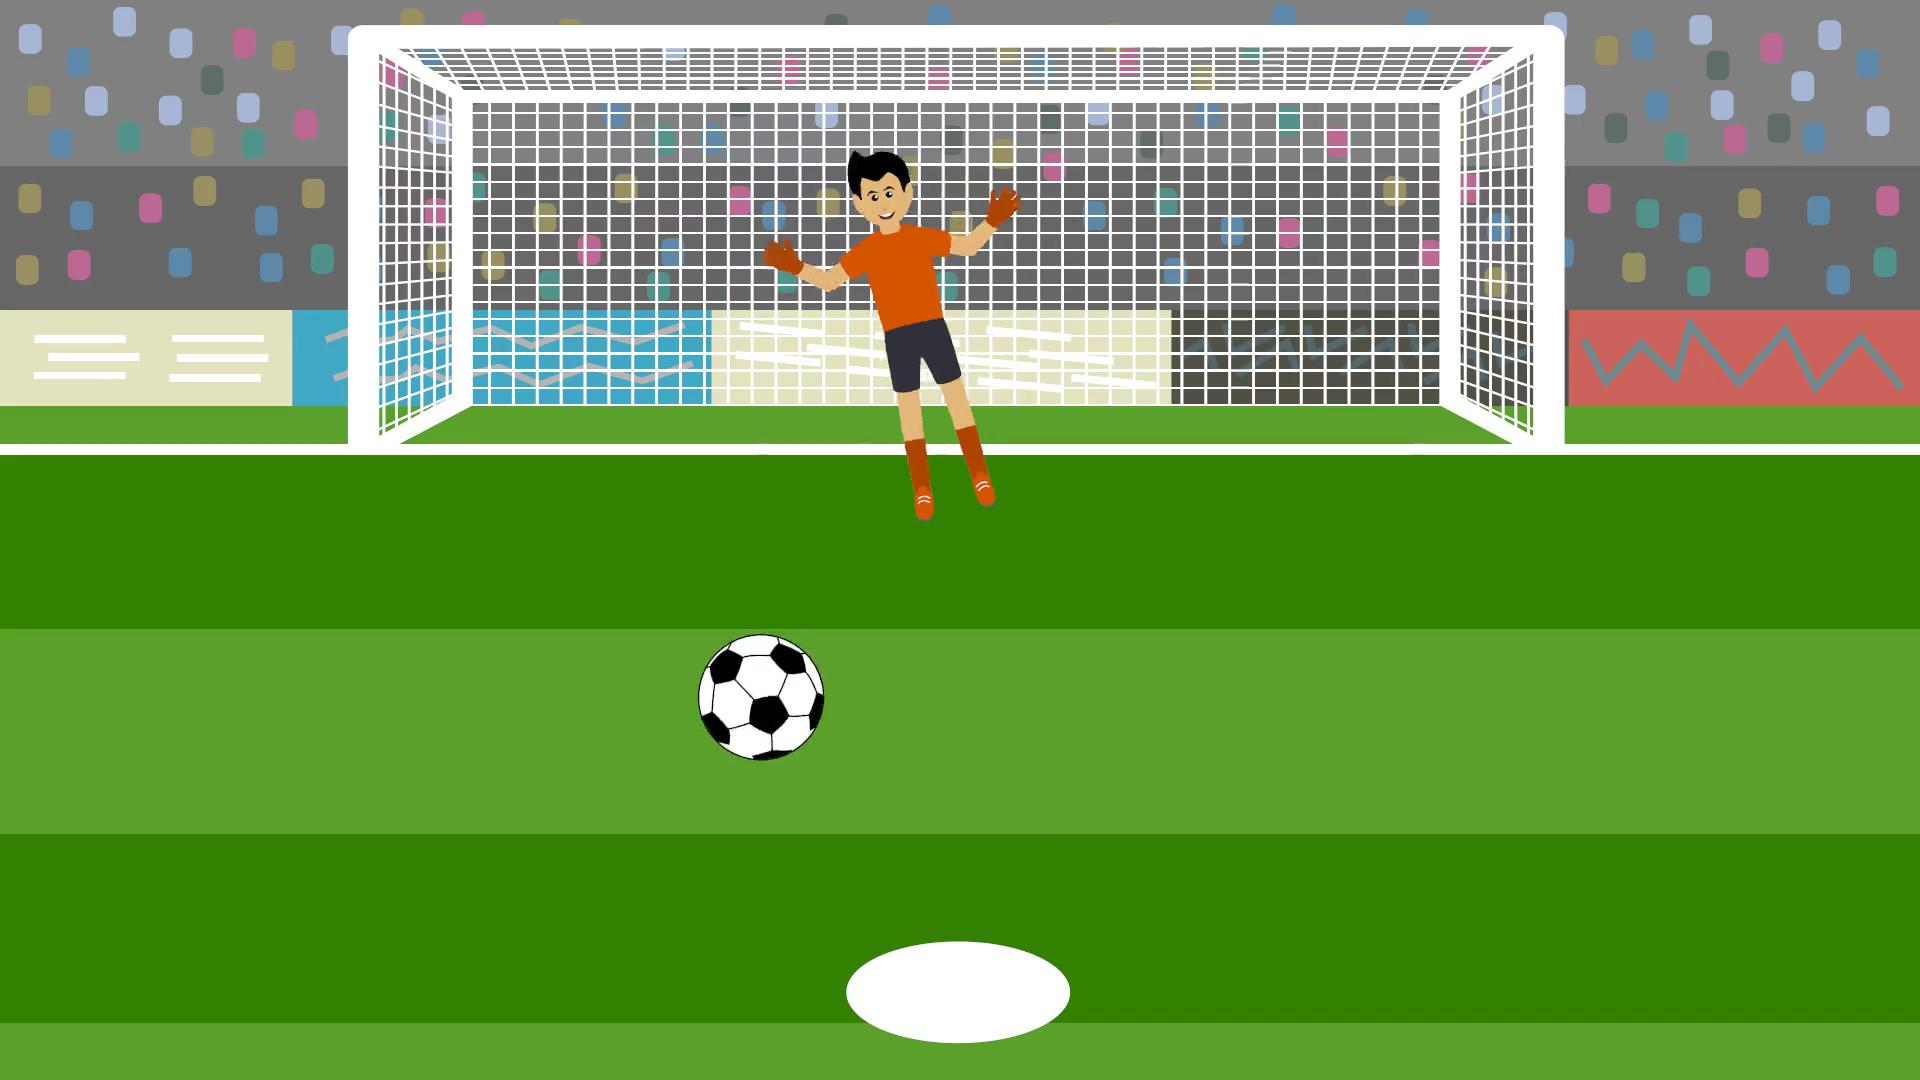
\includegraphics{images/shootout} 

}

\caption{Screenshot of the shootout game}\label{fig:screenshot-shootout}
\end{figure}

\hypertarget{procedure-1}{%
\subsubsection{Procedure}\label{procedure-1}}

The participants played 3 games sequentially against both level-1 and level-2 computer opponents, rather than just one like in the first experiment. Like in the first experiment, the computer opponents retained the same strategy throughout the 3 games, however the participants faced each opponent twice in each game. Specifically, each game was divided into 4 stages numbered 1 to 4, consisting of 20, 20, 10, and 10 rounds respectively for a total of 60 rounds per game. Participants start by facing one of the opponents in stage one, then face the other in stage two. This is repeated in the same order in stages 3 and 4. Which opponent they faced first was counterbalanced. All participants engage in the same three games (namely RPS, FWG and Shootout) in this exact order, and were aware that the opponent was not able to know their choices beforehand but was choosing simultaneously with the player.
In order to encourage participants to think about their next choice, a countdown timer of 3 seconds was introduced at the beginning of each round. During those 3 seconds, participants could not choose an option and had to wait for the timer to run out. A small delay that changed randomly (between 0.5 and 3 seconds) was also introduced in the time it took the AI agent to give back their response, as a way of simulating a real human opponent thinking time. After each round, the participants were given detailed feedback about their opponent actions as well as whether they won or lost the last round. Further information about the outcome of previous rounds was also visible on the game screen below the feedback area. Throughout each stage, participants could scroll down to recall the history of interaction. The number of wins, losses and ties were clearly shown at the top of the screen for each game, and this scoreboard was reinitialised to zero at the onset of a new stage game.
As in the first experiment, all the games have a unique MSNE consisting of randomising across actions. If participants follow this strategy, or simply don't engage in learning how the opponent plays, they would score 0 on average against both level-1 and level-2 players. Evidence of sustained wins would indicate that participants have learned to exploit patterns in the opponent play.

\hypertarget{results-1}{%
\subsection{Results}\label{results-1}}

The RPS game had the lowest average score per round (M = 0.194, SD = 0.345) followed by FWG (M = 0.27, SD = 0.394) and finally the Shootout game had an adjusted average score in between the two (M = 0.289, SD = 0.326).\footnote{A higher score in shootout is expected as there are 2 out of three possible winning actions, compared to one out of three in RPS and FWG. Indeed, a player not aiming to uncover the opponent's strategy and thus choosing to play randomly should be expected to have on average score per round of 0 in both RPS and FWG, and 0.33 in the Shootout game. To make the scores more comparable, and because we are interested in player's performance that is not due to chance, we will adjust all scores in the shootout game by subtracting the average score per round of a random strategy (0.33)}. Using parametric t-tests on adjusted scores, we reject the null hypothesis of random play in all three games (RPS: t(49) = 6.26, \(p\) \textless{} 0.0001 ; FWG: t(49) = 7.25 , \(p\) \textless{} 0.0001 ; Shootout: t(49) = 13.61, \(p\) \textless{} 0.0001 ). Using the average scores obtained by participants in each game and interaction, we explore whether learning has occurred within and between games. We perform a two (condition: level-1 first, level-2 first) by two ( opponent type: level-1 or level-2) by three (game: RPS, FWG, Shootout) by two (interaction: first or second) repeated measures ANOVA with the first factor varying between participants.

\begin{figure}

{\centering 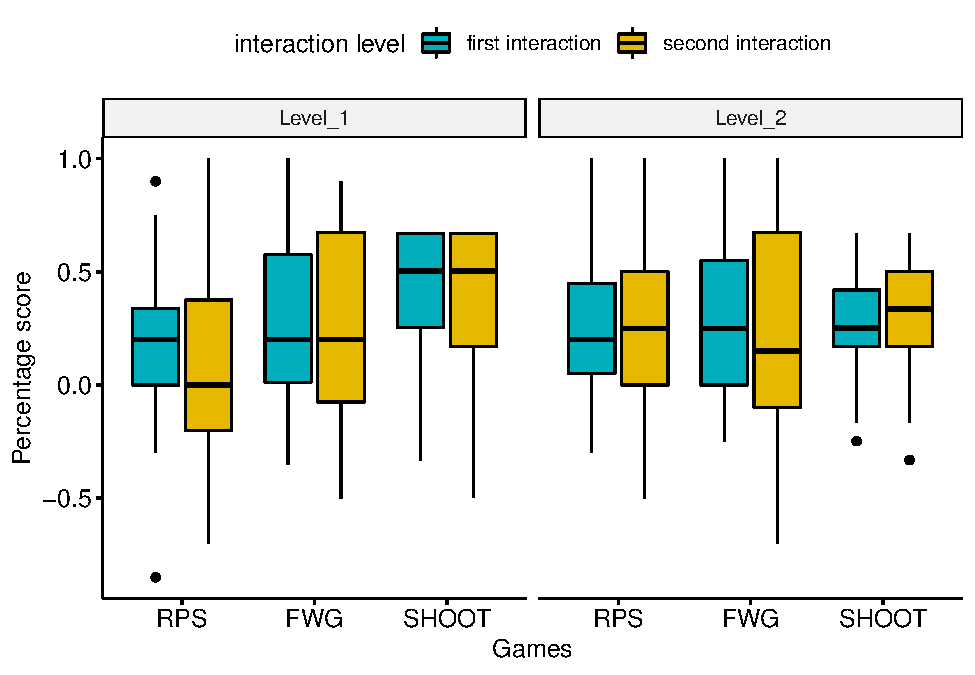
\includegraphics{draft_upgrade_v1_files/figure-latex/exp2-score-by-opp-1} 

}

\caption{Boxplot of scores per game and interaction by opponent type}\label{fig:exp2-score-by-opp}
\end{figure}

There is evidence for a main effect of Game on scores (F(1.85,88.7) = 11.81, \(\eta^{2}\) = 0.04, p \textless{} .0001). To explore these differences further, we look at post-hoc analyses for pairwise comparisons between game scores (p-values adjusted using Holm method for multiple comparisons). We find the performance in the games increases steadily throughout the experiment, with FWG performance significantly higher than RPS (t(96) =2.53, p = 0.025), and performance in the Shootout game also significantly higher than in FWG ( t(96) = 2.32, p = 0.025 ). There was no main effect of either opponent type, the interaction factor( first or second time opponent was faced) , or the condition factor (whether level-1 or level-2 opponent was faced first). There was however a significant interaction effect between Game and opponent type ( F(1.7, 81.82) = 5.31,\(\eta^{2}\) = 0.02, p = .01).
Figure~\ref{fig:exp2-score-by-opp} shows boxplots of game scores, averaged across participants, by game and opponent type. We also distinguish between scores from the first time the players faced the opponent (first interaction) and the second time they did (second interaction). We see that when facing level-1 agents, scores increase steadily after each game, with FWG score significantly higher than RPS ( t(191) = 2.70, p = 0.03) and Shootout scores in turn significantly higher than FWG ( t(191) = 3.05, p = 0.01). There was no significant difference between average scores on any two games when facing level-2 agents however.

\hypertarget{learning-transfer-1}{%
\subsubsection{Learning transfer}\label{learning-transfer-1}}

As a measure for learning transfer we will again compare scores only on rounds 2-6 of each game, excluding the very first round where play is necessarily random.



\begin{figure}

{\centering 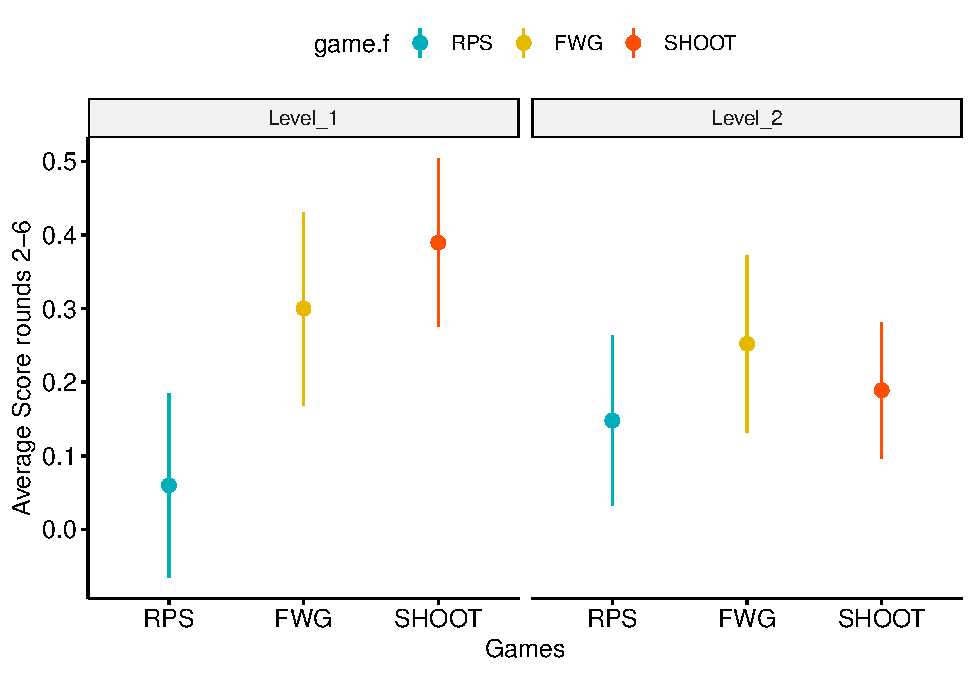
\includegraphics{draft_upgrade_v1_files/figure-latex/exp2-early-scores-1} 

}

\caption{Average early round scores and 95\% confidence intervals by game and opponent for experiment 2}\label{fig:exp2-early-scores}
\end{figure}

In Figure~\ref{fig:exp2-early-scores}, we show the average score across participants and its \(95\) percent confidence interval in rounds 2-6 of the first interaction with the opponent for each game. These scores are also averaged across the levels of condition (meaning they are irrespective of which opponent players faced first). For both the FWG and Shootout games, score in the early rounds of the first interaction are significantly higher than 0 for both opponent types. (Level-1 opponent: FWG: t(270) = 4.99, p \textless{} 0.0001; Shootout: t(270) = 6.66, p \textless{} 0.0001; Level-2 opponent: FWG: t(270) = 4.40, p \textless{} 0.0001; Shootout: t(270) = 3.21, p =0.004 ).

\hypertarget{experiment-2-discussion}{%
\subsubsection{Experiment 2 discussion:}\label{experiment-2-discussion}}

Looking at learning transfer by type of opponent faced, we confirm the result from the first experiment that it is easier to transfer learning to the more dissimilar game (Shootout) when facing a level 1 opponent. Indeed, while the early scores of FWG for level-1 and level-2 facing players are not significantly different from each other, the score of the players facing the level-1 opponent is indeed almost 0.2 point per round higher than that of players facing level-2 opponents, and the difference is statistically significant ( t(144) = 2.45 , p = 0.01). These early scores have also been adjusted to account for the fact that the shootout game has higher average scores when playing randomly, and therefore this difference is really due to better learning transfer and not due to chance.

\newpage

\hypertarget{computational-modelling}{%
\section{Computational modelling}\label{computational-modelling}}

To gain more insight into how participants played the games against the computer opponents, we estimated and compared different computational models of strategies the players may have been using to learn how to beat the opponent. The baseline model assumes play is random, and each potential action is chosen with equal probability. Note that this corresponds to the Nash equilibrium strategy. In this section, we will go through the various models we have used and explain how they update what they learn about the game or the opponent

\hypertarget{reinforcement-learning}{%
\subsection{Reinforcement Learning}\label{reinforcement-learning}}

We include for comparison purposes a simple model-free reinforcement learning algorithm, that reinforces actions that have led to positive rewards, and conversely lowers the likelihood of choosing actions that led to a negative reward, irrespective of any state. We will use a simple delta learning update rule:

\[ V_{t+1}(a) = V_{t}(a) + \alpha \times ( R_{t}  - V_{t}(a)) \]

Where \(V_{t}(a)\) is the value associated with action \(a\) at time \(t\), \(\alpha\) is the learning rate and \(R_{t}\) the reward at time t. The probability of player \(i\) choosing action \(j\) at time \(t+1\) denoted by \(P_{i}^{j}(t+1)\) is based on action values using a softmax choice rule:

\[P_{i}^{j}(t+1) = \frac{e^{\lambda . V_{t}^{j}(a)}}{\sum_{k=1}^{m_{i}}e^{\lambda . V_{t}^{k}(a)}} \]

We extend this very simple model by adding a state space that consists of last round human and agent play. This is akin to using a Q-learning algorithm (Watkins \& Dayan, 1992). The update rule becomes:

\[ Q^{new}(s_{t},a_{t}) = Q(s_{t},a_{t}) + \alpha \times( R_{t}  + \gamma \times \underset{a}{\max}Q(s_{t+1},a) - Q(s_{t},a_{t}) ) \]

Where \(Q(s_{t},a_{t})\) is the value of taking action \(a\) when in state \(s\) at time \(t\), \(\gamma\) is the discount rate applied to future rewards. For instance, \(Q(RS,P)\) denotes the value of taking action \enquote{Paper} this round if the player's last action was \enquote{Rock} and the opponent played \enquote{Scissors}. This is a much richer model allowing the players to compute the values of actions conditional on past play.

\hypertarget{ewa-models}{%
\subsection{EWA Models}\label{ewa-models}}

Next, we use a self-tuning Experience Weighted attraction model (Ho, Camerer, \& Chong, 2004). EWA models particularity is that they nest two seemingly different approaches, namely reinforcement learning and belief learning. Belief based models are based on the assumption that players keep track of the frequency of past plays and best respond to that. In contrast, reinforcement learning does not take into account beliefs about other players, but is such that an action followed by a positive reward is more likely to be repeated than an action followed by a negative reward. The self-tuning EWA model has been shown to perform better than both these nested models in multiple repeated games and has the advantage of having only one free parameter, the inverse temperature in the softmax choice function.
Let's define some notation in order to write the update rule of the self-tuning EWA model. For player i, there are \(m_{i}\) strategies, denoted \(s_{i}^{j}\) (i.e player i's strategy number j). Strategies actually played by i in period t, are denoted \(s_{i}(t)\), while the opponent's strategy at time t is denoted \(s_{-i}(t)\). After playing \(s_{i}^{j}\) at time \(t\), player i pay-off is denoted \(\pi_{i}(s_{i}^{j},s_{-i}(t))\), and the actual pay-off the player received is \(\pi_{i}(t)\).
The EWA model is based on updating \enquote{Attractions} for each action over time. For instance, the attraction of strategy \(j\) to player \(i\) at time \(t\) is written \(A_{i}^{j}(t)\). Future action choice probabilities are based on these attractions using the softmax playing rule:

\[P_{i}^{j}(t+1) = \frac{e^{\lambda  A_{i}^{j}(t)}}{\sum_{k=1}^{m_{i}}e^{\lambda A_{i}^{k}(t)}} \]

The attractions are updated over every time step \(t\) using the following update rule :

\[ A_{i}^{j}(t) =  \frac{\phi \times N(t-1) \times A_{i}^{j}(t-1) + [ \delta + (1-\delta) \times I(s_{i}^{j},s_{i}(t))] \times \pi_{i}(s_{i}^{j},s_{-i}(t)) } {\phi \times N(t-1) + 1} \]

Here, \(I(x,y)\) is the indicator function equal to 1 if \(x = y\) and 0 otherwise. A simple way to think about this update rule is that attractions are multiplied by a parameter that represents experience (\(N(t-1)\)) which is itself decaying by a weight \(\phi\). The result is added to either the pay-off received (when the indicator function is 0), or to \(\delta\) times the foregone pay-off (when indicator function is 1). We can see that setting \(\delta = 0\) leads to reinforcement of past actions, while positive and high delta parameters make the update rule take into account foregone pay-offs, which is similar to weighted fictitious play (Cheung \& Friedman, 1994). While the assumption in expanding the update rule above is that \(\phi\) and \(\delta\) are free parameters (Camerer, Ho, \& Others, 1997), the self-tuning aspect of the model comes from the fact that these are now self-tuned using the formulas expanded in (Ho et al., 2004).

\hypertarget{tom-models}{%
\subsection{ToM models}\label{tom-models}}

In this set of models, we assume that participants start with a prior belief that the opponent is a level-k agent, with uniform probability of the level \(k \in \{ 0, 1, 2\}\), and use evidence of past play to update their beliefs in a Bayesian way about the true value of k. More formally, if we define \(D_{t}\) as data available at time \(t\) then the probability of the opponent being a level-k is updated using:

\[ P(level=k | D_{t})  \propto  P(D_{t}|level=k ) \times P(level=k)\]

These models also assume the opponent can deviate from these level-k strategies and play randomly with probability \(\theta\), a parameter to be fit. We also assume that participants base their actions on their beliefs about the level of the opponent, so actions get chosen probabilistically using a softamx choice rule with probabilities of each opponent level as inputs. We distinguish between multiple ToM models based on their ability to keep what was learned about the opponent in memory and hence facilitate transfer. In a No-Between-Transfer (NBT) model, players have no memory of what was learned about the opponent and start every new game assuming each level-k has equal probability. In the context of Experiment 2 where players face both opponents, this model assumes that participants transfer learning within the same game, from the first to the second interaction with the opponent, but are not able to transfer that learning to new games (within but no between transfer).Conversely, In a Between-Transfer model (BT), players are assumed to keep in memory what was learned about the type of opponent faced (vector of probabilities of level-k) and use that at the beginning of each new game. In the context of experiment 2, we still assume that if between transfer is present, then within game transfer is also present (from first to second interaction). In experiment two, on top of these two models, we fit another model in which all stages of the game and all new games start with a fresh uniform probability of level-k opponent (NT), so no within or between opponent model learning transfer.

\hypertarget{estimation-and-model-comparison}{%
\subsection{Estimation and model comparison}\label{estimation-and-model-comparison}}

In both experiments, all models were fit to each participant data, with optimal parameters being estimated using maximum likelihood. Using information criteria based Bayesian model comparison (BIC), the best fitting model for each participant was chosen and we compared the number of participants whose behavior was best explained by each model.

In experiment 1, we fit a total of 5 models: A baseline model assuming random play (Nash), a Bayesian Theory of mind model allowing transfer betwen games (TOM\_BT) and another with no transfer between games (TOM\_NBT), as well as a Q-learning model with state space consisting of last round play (QL\_states), and finally a self tuning EWA model with the same state space (STEWA\_states). In experiment 2, because participants were interacting with each opponent twice within each game, we allowed models to transfer learning within games between the first and second interactions. Therefore on top of the two ToM models mentionned above (ToM\_BT and Tom\_NBT), we also allow the Q-learning model with states to either have the ability to transfer learning between the first and second interaction (QLS\_Tr) or not (QLS\_NT). Likewise, we fit both a self tuning EWA model with transfer between stages of the same game (STEWA\_Tr) or without transfer (STEWA\_NT). Counting the base model wiht random play (Nash) we therefore fit a total of 8 models in experiment 2.

\hypertarget{experiment-1-modelling}{%
\subsection{Experiment 1 modelling :}\label{experiment-1-modelling}}

Figure~\ref{fig:exp1-comp-models} shows the results for experiment 1: we can see that while some participant's learning behavior was either random or explained by some of the base models, a significant number of participants in experiment one had learning most consistent with Q-learning with states defined by last round play.
Table ~\ref{tab:exp1weightstable} shows the model BIC weights as well as the number of participants best fit by each model.

\begin{table}[tbp]
\begin{center}
\begin{threeparttable}
\caption{\label{tab:exp1weightstable}Experiment one Average BIC weights and number of participants best fit by model}
\begin{tabular}{llllll}
\toprule
 & \multicolumn{1}{c}{Nash} & \multicolumn{1}{c}{ToM\_BT} & \multicolumn{1}{c}{ToM\_NBT} & \multicolumn{1}{c}{QL\_states} & \multicolumn{1}{c}{STEWA\_States}\\
\midrule
Model BIC weights & 0.10 & 0.07 & 0.05 & 0.73 & 0.05\\
Count best fit & 8.00 & 1.00 & 3.00 & 39.00 & 1.00\\
\bottomrule
\end{tabular}
\end{threeparttable}
\end{center}
\end{table}

\begin{figure}

{\centering 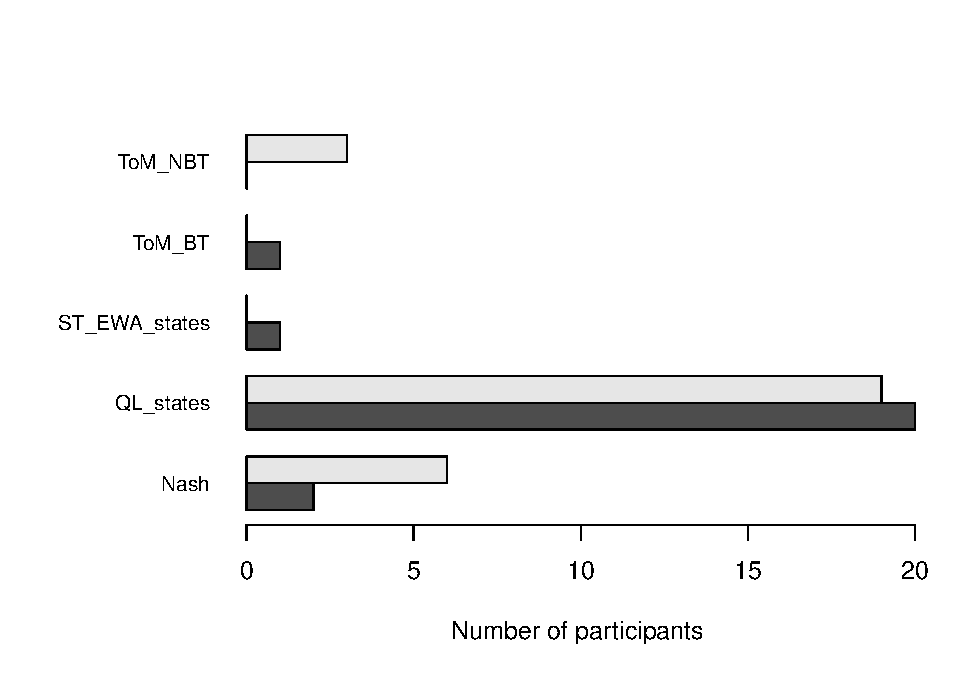
\includegraphics{draft_upgrade_v1_files/figure-latex/exp1-comp-models-1} 

}

\caption{Experiment 1 - Histogram of best fitting computational models by condition}\label{fig:exp1-comp-models}
\end{figure}

Next we compared the performance of players whose actions are best fit by each of our hypothesized models. Figure~\ref{fig:exp1-cumScores} shows the average cumulative performance of players across games, for participants grouped by which model best fits their behavior in experiment 1. We can see that participants whose actions are most consistent with learning a ToM opponent model in a Bayesian way had the best overall performance (without transfer), followed by Q-learning conditional on last round play. EWA, QL and random players had, understandably the lowest performance.

\begin{figure}

{\centering 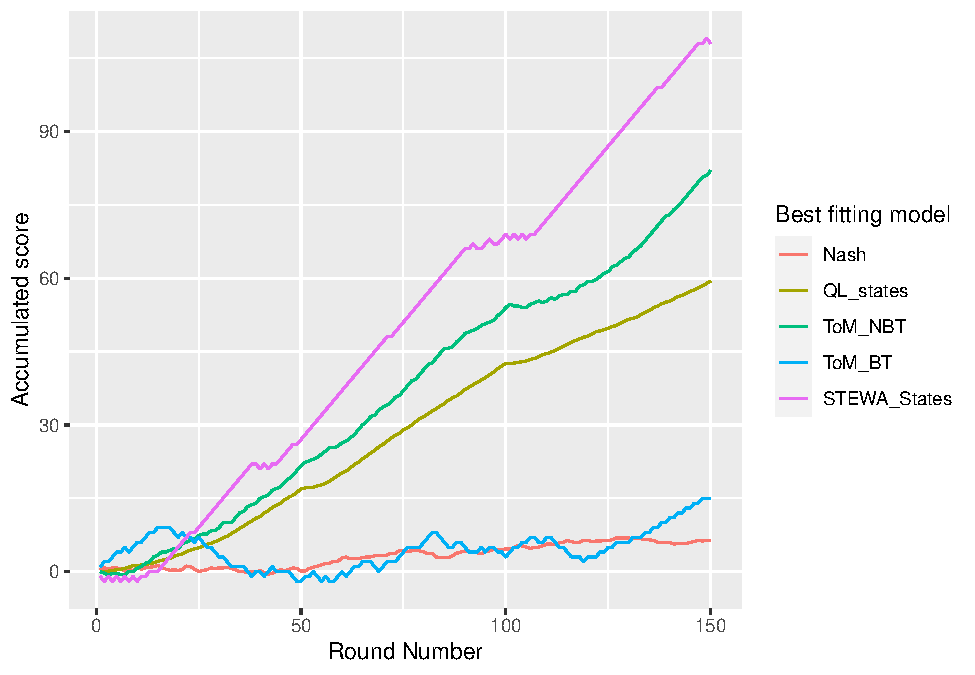
\includegraphics{draft_upgrade_v1_files/figure-latex/exp1-cumScores-1} 

}

\caption{Experiment 1 - Average cumulative scores of participants by best fitting model}\label{fig:exp1-cumScores}
\end{figure}

\hypertarget{experiment-2-1}{%
\subsection{Experiment 2}\label{experiment-2-1}}

\begin{figure}

{\centering 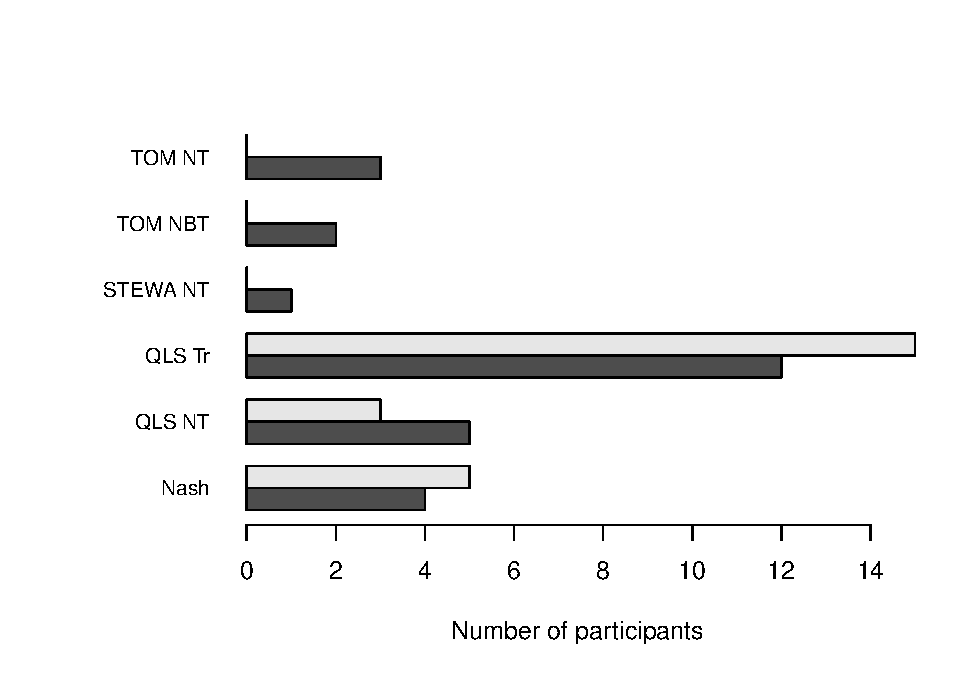
\includegraphics{draft_upgrade_v1_files/figure-latex/exp2-comp-models-1} 

}

\caption{Experiment 2 Histogram of best fitting computational models by condition}\label{fig:exp2-comp-models}
\end{figure}



\begin{table}

\caption{\label{tab:exp2-weights-table}Experiment 2 - Average BIC weights and number of participants best fit by model}
\centering
\resizebox{\linewidth}{!}{
\begin{tabular}[t]{l|r|r|r|r|r|r|r|r}
\hline
  & Nash & TOM BT & TOM NBT & TOM NT & QLS NT & QLS Tr & STEWA NT & STEWA Tr\\
\hline
BIC weights & 0.13 & 0.02 & 0.06 & 0.06 & 0.18 & 0.49 & 0.04 & 0.03\\
\hline
Count best fit & 9.00 & 0.00 & 2.00 & 3.00 & 8.00 & 27.00 & 1.00 & 0.00\\
\hline
\end{tabular}}
\end{table}

In experiment 2, we can see from Figure~\ref{fig:exp2-comp-models} that Q-learning with the aforementioned state-space was again more successful than the Bayesian models in fitting player's action choices. In experiment 2 when participants faced both level-1 and level-2 agents sequentially, the Bayesian models (with or without transfer) did not fit players observed data as well. This is also reflected in BIC weights in Table ~\ref{tab:exp2-weights-table}

\begin{figure}

{\centering 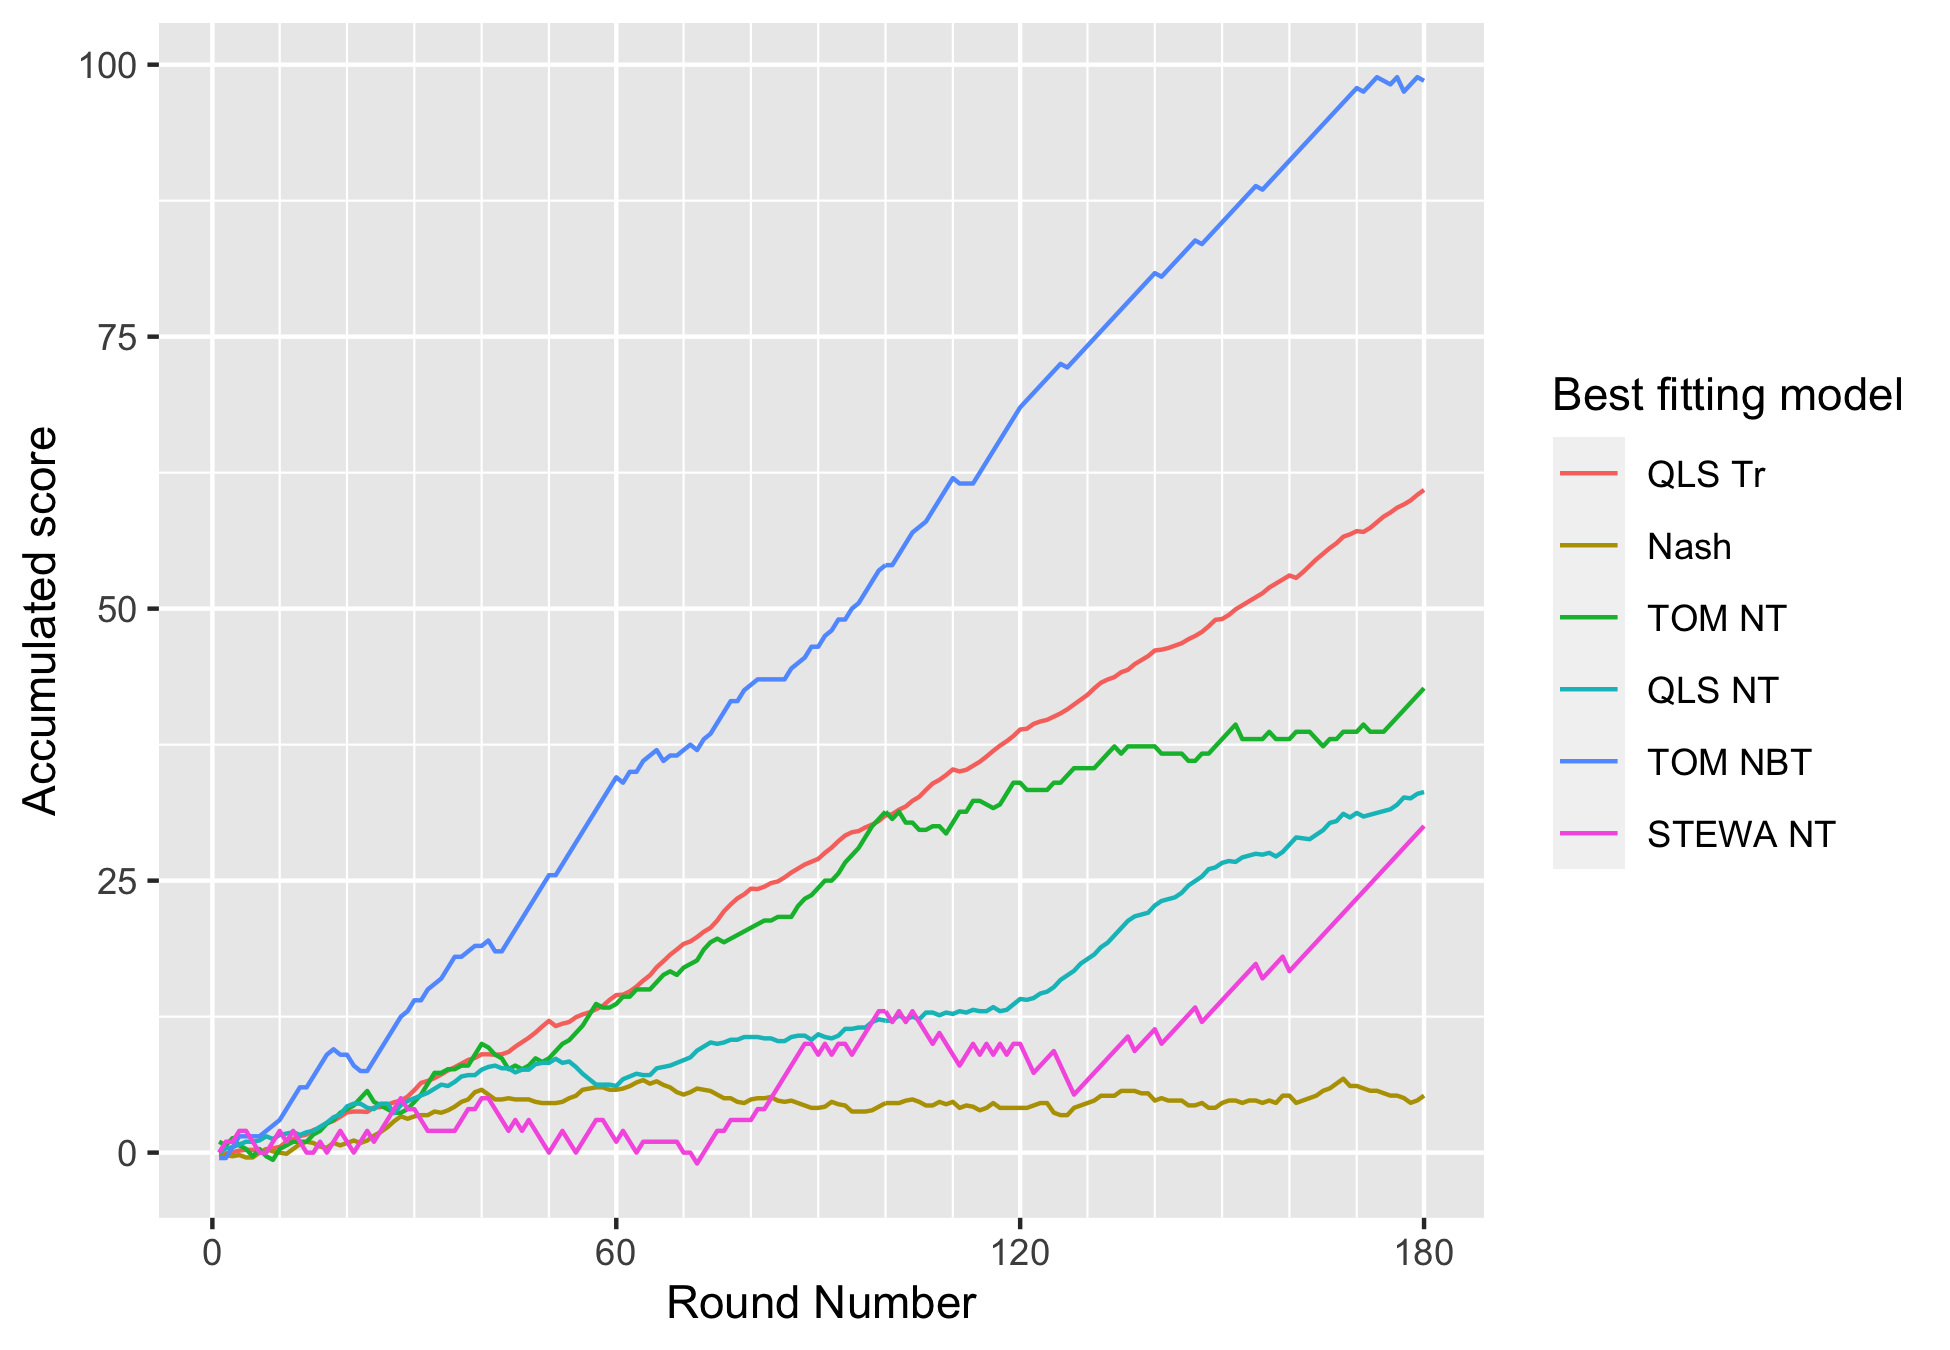
\includegraphics{draft_upgrade_v1_files/figure-latex/exp2-cumScores-1} 

}

\caption{Experiment 2 Average cumulative scores of participants by best fitting model}\label{fig:exp2-cumScores}
\end{figure}

Plotting cumulative scores by best model for experiment 2, we see very similar results looking at Figure~\ref{fig:exp2-cumScores}, in that participants whose behavior was best fit by a ToM model of learning the opponent strategy had the highest cumulative performance. Out of these ToM models, the one in which there is within-game but no between-game transfer (NBT) had the best cumulative performance (although it only fit 2 participants best), followed by a model in which both within and between transfer of opponent models is allowed (BT). The next best model from a performance perspective was a Q-learning model with states and within game transfer, followed by ToM models where players reset opponent models at each stage of each game (NT). As expected, random play was at the bottom of cumulative performance.

\hypertarget{using-hidden-markov-model-to-explore-strategy-switching}{%
\subsection{Using Hidden Markov Model to explore strategy switching}\label{using-hidden-markov-model-to-explore-strategy-switching}}

The computational modelling indicates that most players are best fit by Q-learning type models with states defined by last round play. This is at odds with the findings from the section regarding learning transfer: If indeed most participants use Q-learning with states to choose their actions, then they should not be able to transfer learning to the early rounds of the new game. In order to understand better what is going on, we plot the likelihood by trial for each game and each of the three strategies: Q-learning with states, and Theory of Mind models with and without the possibility of across game transfer.

We start with experiment 1 data. Figure~\ref{fig:exp1-lik-by-tr} shows that in the later games, the likelihood for the ToM models is higher in the initial rounds in which learning transfer is measured, but that over time, the likelihood of Q-learning model becomes more important and exceeds that of ToM models.

\begin{figure}

{\centering 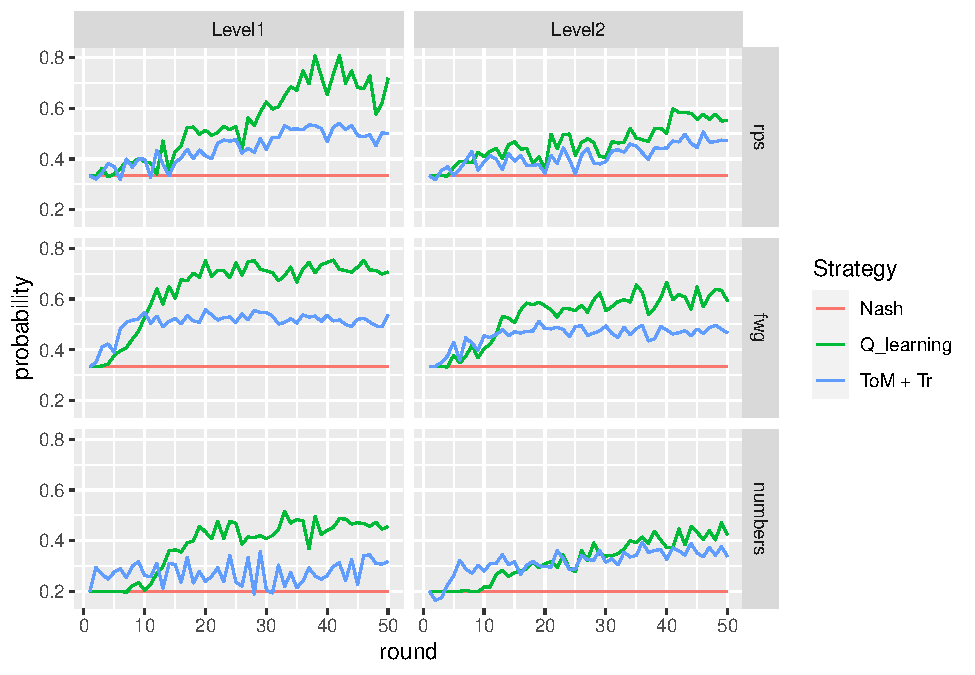
\includegraphics{draft_upgrade_v1_files/figure-latex/exp1-lik-by-tr-1} 

}

\caption{Experiment 1 Likelihood by trial by game and opponent faced}\label{fig:exp1-lik-by-tr}
\end{figure}

Likewise, in experiment 2, we want to understand the dynamic of strategy choice by plotting the likelihood by trial for each strategy, using the optimal parameters found when fitting the model. Figure~\ref{fig:exp2-lik-by-tr} shows that, as in experiment 1, ToM models had higher likelihood in the early stages of the second (most similar) game, however the likelihood of Q-learning with states models increases steadily to be the highest in the later stages of all games. In the third and more dissimilar game, we get a result that is different from experiment 1. In this instance, the likelihoods of the ToM models stay constant and close to their initial values.

\begin{figure}

{\centering 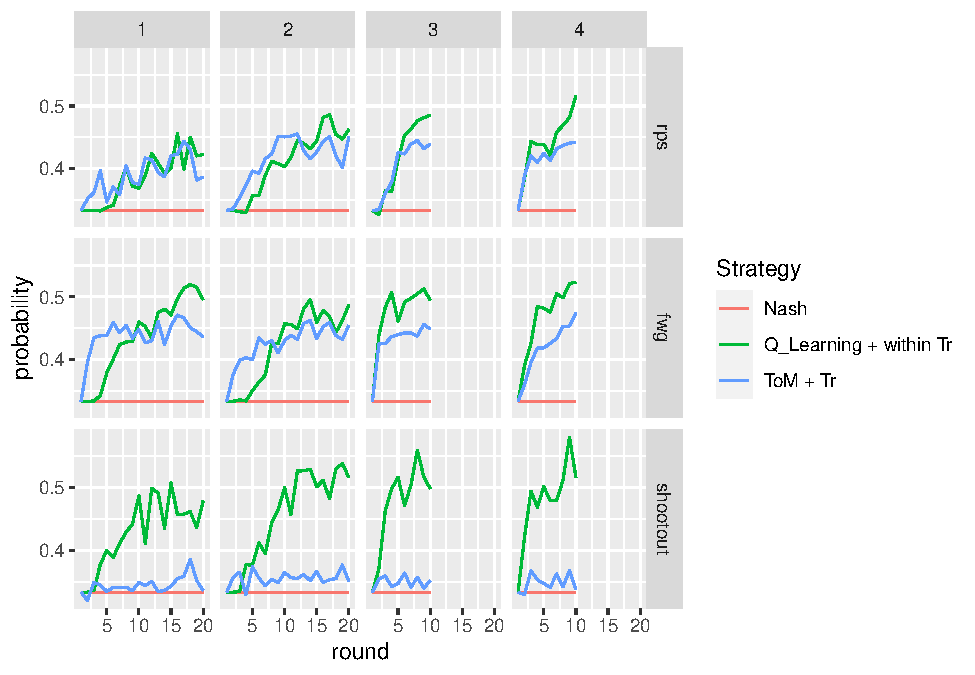
\includegraphics{draft_upgrade_v1_files/figure-latex/exp2-lik-by-tr-1} 

}

\caption{Experiment2 likelihood by trial by game and opponent faced}\label{fig:exp2-lik-by-tr}
\end{figure}

The fact that the likelihoods of the main strategies considered cross over in both experiments could be interpreted as indicative of participants switching between strategies as the games progressed. Indeed, in both experiments, following our results, it seems that in the earlier stages of the latter games, the ToM based strategies fitted observed action choices better than Q-learning based ones, with a reversal of the roles in later stages.

In order to test for the existence of strategy switching in participants' play, we fit Hidden Markov Models in which the latent states are the 3 strategies used (Q-learning with state space consisting of previous round play, ToM based model with opponent model transfer, and a base model consisting of random play consistent with a Nash equilibrium strategy). Hidden Markov models are useful tools to explore structure in observed time series. They are named as such because of two properties: First, they make the assumption that any observable action at time t results from a process whose state at time t , named \(S_{t}\) is \enquote{hidden} from the observer. Second, it also assumes that this hidden process has a Markov property, meaning that given state \(S_{t-1}\), the value of \(S_{t}\) is independent of all states occurring before time \(t-1\). We also assume that \(S_{t}\) has a discrete probability distribution in that it take one of K discrete values. The model is therefore specified by initial probabilities of being in each state \({1,2,...,K}\) and transition probabilities for moving from state \(i\) to state \(j\). These probabilities are fit using observed actions generated from these hidden states.

To investigate the possibility of strategy switching, we fit two different hidden Markov models with the depmixS4 R package. In the first model, we allow for a non-nil probability of players transitioning from one state (strategy) to another. In the second model, we assume that such switching does not happen, and as such assume implicitly that when players start with a particular strategy, they continue using it throughout the experiment. We then compare the likelihoods of each HMM model using a likelihood ratio test.

\hypertarget{experiment-1-1}{%
\subsubsection{Experiment 1:}\label{experiment-1-1}}

\begin{figure}

{\centering 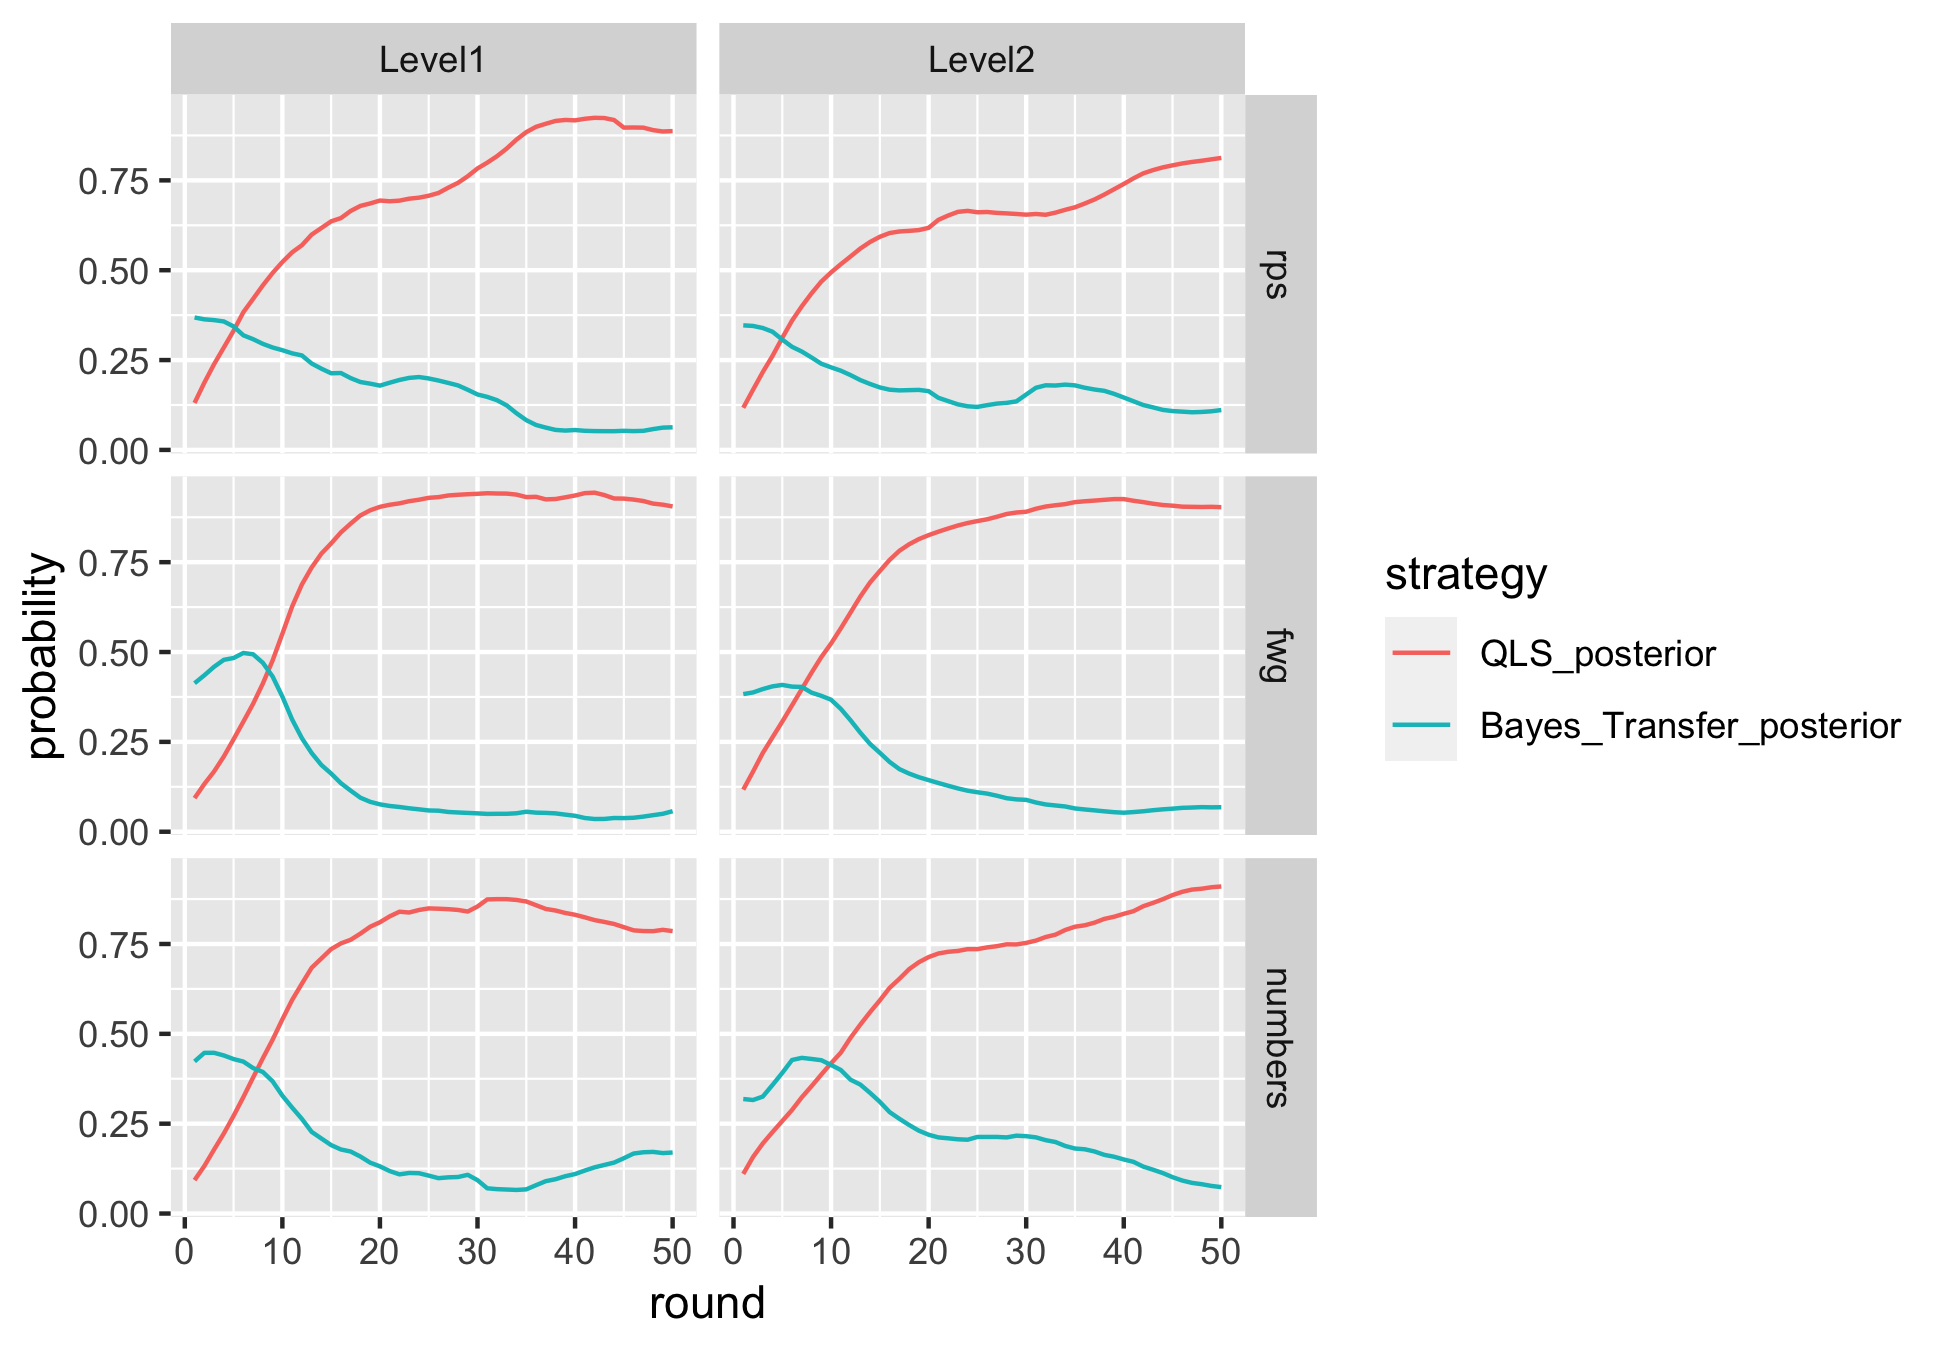
\includegraphics{draft_upgrade_v1_files/figure-latex/exp1-posteriors-plot-1} 

}

\caption{Experiment1 posterior probability of strategies by game and opponent faced}\label{fig:exp1-posteriors-plot}
\end{figure}

In experiment 1, the HMM model with switching fits significantly better than the non-switching one (\(p < .001\)). This is further statistical evidence in favour of the hypothesis that participants switch between strategies. In order to understand at which stage of the games the switching might happen, and whether there are any differences between games and type of opponents faced, we plot in Figure~\ref{fig:exp1-posteriors-plot} the average (across participants) posterior probabilities of each state (strategy), as a function of trial and opponent faced. The posterior probability is the probability that an observation comes from a component distribution a posteriori, i.e.~given the value of the observation. In the first experiment, we can see from the plots of FWG and numbers games for level-1 opponent that although the likelihoods are very close, the posterior probability of the Bayesian model with transfer is slightly higher than that of the QLS model in the very early rounds, but decreases rapidly while the posterior probability of the QL-learning with states models keeps increasing.

\hypertarget{experiment-2-2}{%
\subsubsection{Experiment 2:}\label{experiment-2-2}}

\begin{figure}

{\centering 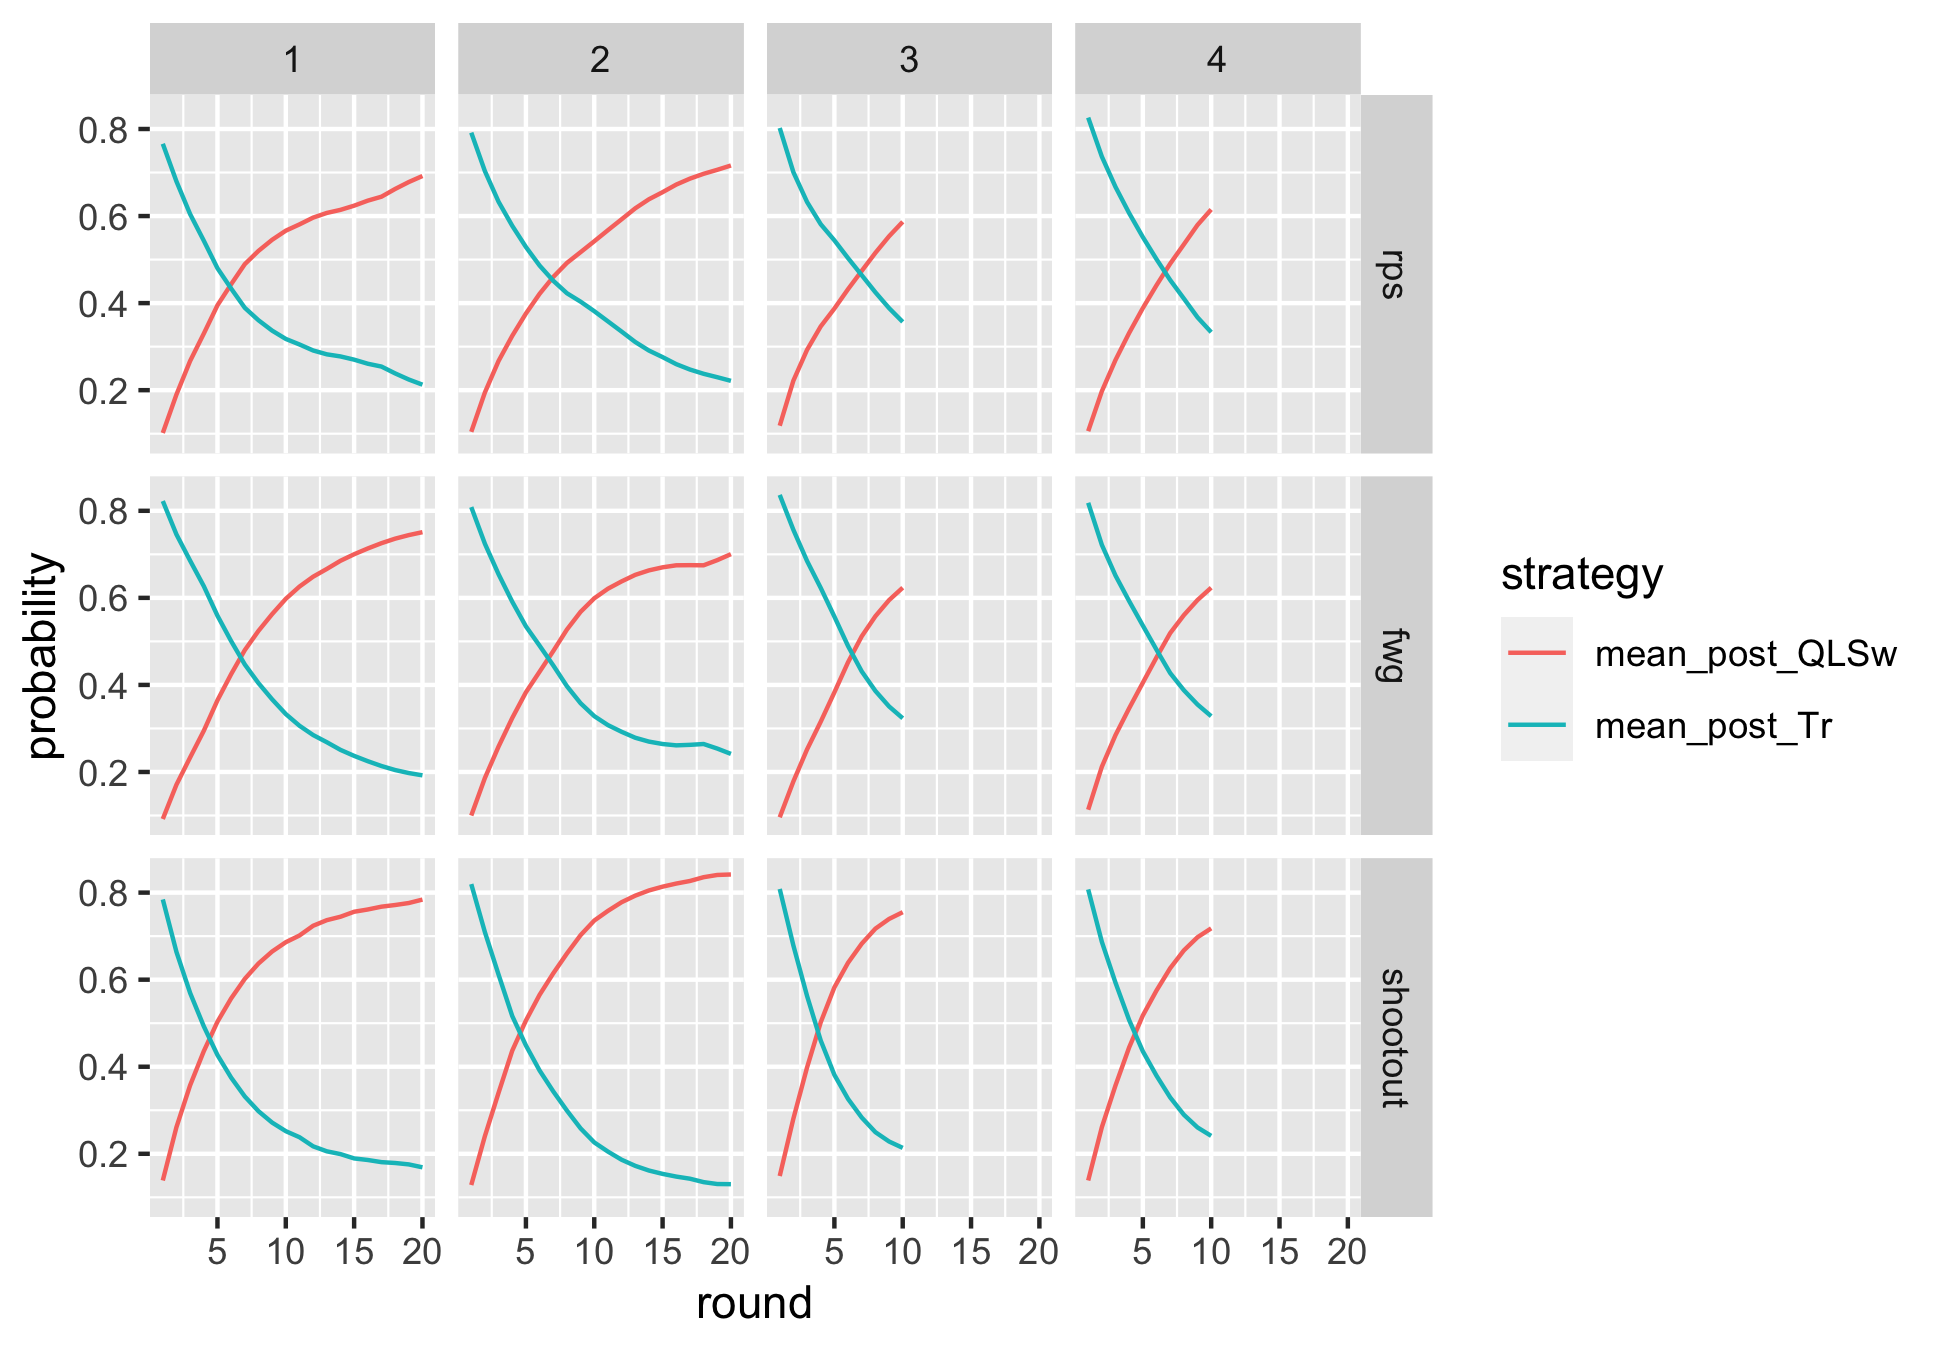
\includegraphics{draft_upgrade_v1_files/figure-latex/exp2-posteriors-plot-1} 

}

\caption{Experiment2 likelihood by trial by game and opponent faced}\label{fig:exp2-posteriors-plot}
\end{figure}

The switching model in experiment two has also significantly higher likelihood (\(p\) = 0.00). On top of indications from looking at the likelihood by trial graphs, we have therefore further evidence that participants did indeed switch their strategies as the games progressed. The posterior probability plot in Figure~\ref{fig:exp2-posteriors-plot} shows switching much more clearly across games and stages. The switching also seems to happen very early on at the beginning of each game and stage, and is also consistently in the same direction: The probability of Bayesian models with transfer being initially high, then decreasing rapidly while the posterior probability of QL-Learning with states and within transfer learning increases rapidly.

Therefore, HMM modelling shows clear evidence in favour of strategy switching by participants, specifically after a few rounds of play. The strategy switching is consistently from ToM models towards Q-learning with states models in both experiments.

\newpage

\hypertarget{discussion}{%
\section{Discussion}\label{discussion}}

In this study, we investigated human learning transfer across games by making human participants play against computer agents with rule-based level-k strategies. We were interested in exploring whether participants learn about the strategy of their opponent and transfer such knowledge between games, and whether this is modulated by the similarity between games and the sophistication of the agent.

The results of our first experiment show that the majority of participants learn to adapt to the opponent strategy over multiple interactions and generalise this learning to the similar game. We used results on very early rounds for measuring transfer as they are unlikely to be tainted by any within game learning. Using this approach, we showed that transfer to the more dissimilar game was modulated by the degree of sophistication of the agent, with evidence for transfer when players face the less sophisticated agent but not the more sophisticated one.

In the second online experiment, there were many more opportunities to test transfer than before: 2 opportunities to transfer opponent models within each game, and a total of three games, which means 6 opportunities to test transfer. The results on learning transfer confirmed prior findings from the first experiment. While there was no evidence of higher scores across interactions within the same game (likely due to the lower number of rounds per interaction and the higher cognitive load of facing two opponents rather than one), we found evidence for learning transfer across games as early round scores analysis confirmed. We also found that learning transfer is modulated by the type of opponent faced. When the players faced the level-1 opponent, they were able to transfer learning. However, when they faced the level-2 opponent, there was weaker evidence for transfer. The lack of transfer when facing the more sophisticated opponent might be due to the difficulty of learning that opponent strategy to start with. A player cannot transfer what they have not learnt and as such, since it might be harder to learn the strategy of the level-2 opponent, this in turn might translate into weaker evidence for transfer.

Coming back to learning transfer, we observed evidence that participants start off new games with prior knowledge as their scores are significantly higher than chance, confirmed both by early stage analysis as well as rounds 2-6 scores analysis. The question we ask ourselves therefore is: What exactly did the players learn in RPS that allowed them to beat the opponent in FWG and Shootout? what did the players learn specifically about the opponent strategy and what form did this learning take?

We will proceed by considering multiple potential answers to this question. A possible hypothesis for learning the opponent's strategy is the use of simple rules based on last round play (for instance, I play scissors whenever opponent played rock in last round, or whenever the last round play was rock/scissors, I should play paper in this round, etc\ldots{}). Our Q-learning with states as prior-round play model is a good proxy for this type of strategies. While this approach certainly seemed to be the best fit for many player's behavior, it is unsatisfactory in explaining some of the learning transfer evidence we showed. Indeed, learning the best action in a particular state is not transferable to a new game since the state space is different and there is no single mapping between the state spaces of the initial and latter games. These rules would therefore need to be learned anew in the latter game which is inconsistent with above chance performance in very early rounds.

Likewise, assuming that players learn a complete model of the environment (for instance the transition probabilities from last round play to new play) might explain learning within games but is equally unable to account for early games transfer of learning as such models, besides being cognitively very expensive to learn, would require many rounds of practice. Another issue with these hypotheses is that they are not consistent with significant score differences between those facing level-2 and level-1 opponents. More specifically, if we assume that participants were using some type of associative learning or relying on spatial heuristics, then their scores should not depend on the degree of strategic sophistication of the opponent since their approaches would render this variable irrelevant. To be sure, if a participant learns to pick say \enquote{scissors} whenever the opponent last picked \enquote{rock}, then the degree of strategic sophistication of the opponent (its level k) should not impact this learning, and we would expect in this case there would be no difference between scores when facing level-1 and level-2 opponents, which is not the case here. The fact that the degree of sophistication of the opponent matters points to the importance of opponent modelling to successful transfer of learning.

We are left with two possible explanations: First, it is possible that the players have uncovered a heuristic that allows them to beat the opponent without explicitly modelling their strategy, and is robust to transfer. Indeed, because of the cyclicality in action choices (e.g : Rock beats Scissors beats Paper beats Rock), it is possible to beat level-2 opponents most of the time by following a simple rule: Play in the next round whatever the opponent played in the last round. This is a rule that wins and is also robust to transfer as it does not depend on action labels and even works in the dissimilar game.

The second explanation of learning transfer is that it is driven by a group of participants that are able to build a mental representation of what the strategy of the opponent is. A successful mental representation would take the perspective of the opponent or endow it with intentionality in order to detect its strategy when the opponent is playing based on a level-k reasoning model. For instance, the player may think \enquote{My opponent is always trying to be one step ahead of me, therefore, I will be one step ahead of where it thinks I will be}. This mental representation would facilitate the use of theory of mind abilities and thus enable the players to learn opponent strategies when they are based on human-like reasoning models such as level-k or cognitive hierarchy. This type of learning would be deemed \enquote{explicit} in the psychology literature as a process through which knowledge consists of cognitive representations of concepts and rules, as well as the relationship between them. It involves the evaluation of explicit hypotheses and results in better problem-solving skills (Mandler, 2004). Since it is less context dependent, this type of learning is generalizable to new situations, akin to the more general framework of rule-based learning explored by Stahl (2000, 2003).

Our second experimental design allows us to test whether the first explanation holds. Since there is a simple transferable heuristic that works against level-2 players, and since as far as we know, there are no similar ones against level-1 players, if indeed participants were using this, they would perform better and transfer learning more easily when facing level-2 opponents. Because level-2 opponents use a higher level of strategic reasoning, they should in fact be harder to play against and in the absence of such a heuristic, performance and learning transfer should be worse.

Our results show that in fact, it was harder to transfer learning when facing level-2 opponents, both comparing first interactions across games and using early rounds analysis. Based on our assumptions, we conclude therefore that the most likely explanation is that participants who are able to beat the opponent and transfer learning are likely to be explicitly modelling the opponent strategy using level-k reasoning, compared to using simple learning rules they uncovered during the course of learning.

Our computational modelling allowed us to delve deeper into what might be driving the observed learning transfer. Initial modelling of observations using all available data seems to indicate that the most likely model was a Q-learning type model. However, as we argued above, that would be inconsistent with the evidence for learning transfer. Breaking down likelihoods by trial and fitting a hidden Markov model to the data with states being the various strategies that participants are assumed to be using, we showed evidence for within game switching of strategies. Participants start the early rounds of a new game acting in a way consistent with a Bayesian Theory of mind level, which would be accurate and generalisable but computationally expensive. However, as trials continue, participants seem to switch to a habitual type of learning (QL-models).

Why is this switching happening? We believe that participants show flexibility in their use of learning strategies. When a new game is started that is similar to a previously played game with the same opponent, participants need a way to transfer prior knowledge of the opponent and apply it to the new game in order to best respond. Adopting a Bayesian model based on ToM achieves the goal of transferring the opponent model and thus coming up with best responses in the early trials. However, Bayesian ToM models are computationally expensive and require higher order thinking (I think that you think that I think\ldots{}). As such, as the games progresses, they may become burdensome and the higher amount of historical interaction in the new game allows participants to have enough data to start using the cognitively cheaper model-free learning strategies such as Q-learning. The preference for less computationally demanding strategies is well established (Wouter Kool, Joseph T. McGuire, Zev B. Rosen, Matthew M. Bovinick, 2011). Moreover, the ability to flexibly switch is also consistent with evidence from the literature on learning strategies in humans, showing that they indeed shift between model-based and model-free learning when the environment requires it (Simon \& Daw, 2011).

\hypertarget{conclusion}{%
\section{Conclusion}\label{conclusion}}

Our online experiments results are consistent with behavioural game theory findings, in that human players can deviate from Nash equilibrium play and learn to adapt to the opponent strategy and exploit it when the opponent itself is deviating from Nash equilibrium. Moreover, we showed that participants transfer their learning to new games with varying degrees of similarity. The transfer is also moderated by the level of sophistication of the opponent, with participants showing more success in learning and transferring against opponents adopting a less sophisticated strategy.

Having said that, there remains a high degree of heterogeneity between players. There is a high positive association between players who learn to beat the sophisticated and less sophisticated opponents, indicating that some players are more able to detect the patterns in opponent play and learn how to exploit them. Moreover, the computational modelling shows that it is likely that players start each game using a model-based learning strategy that facilitates generalisation and opponent model transfer, but then switch to behaviour that is consistent with a model-free learning strategy as the experiment goes on. This is likely driven by a trade-off between computational complexity and accuracy between model based and model free strategies.
\newpage

\hypertarget{references}{%
\section{References}\label{references}}

\begingroup
\setlength{\parindent}{-0.5in}
\setlength{\leftskip}{0.5in}

\hypertarget{refs}{}
\leavevmode\hypertarget{ref-arad201211}{}%
Arad, A., \& Rubinstein, A. (2012). The 11-20 money request game: A level-k reasoning study. \emph{American Economic Review}, \emph{102}(7), 3561--3573.

\leavevmode\hypertarget{ref-baarslag2016learning}{}%
Baarslag, T., Hendrikx, M. J. C., Hindriks, K. V., \& Jonker, C. M. (2016). Learning about the opponent in automated bilateral negotiation: a comprehensive survey of opponent modeling techniques. \emph{Autonomous Agents and Multi-Agent Systems}, \emph{30}(5), 849--898.

\leavevmode\hypertarget{ref-camerer1997experience}{}%
Camerer, C., Ho, T.-H., \& Others. (1997). \emph{Experience-weighted attraction learning in games: A unifying approach}.

\leavevmode\hypertarget{ref-cheung1994learning}{}%
Cheung, Y.-W., \& Friedman, D. (1994). \emph{Learning in evolutionary games: some laboratory results}. University of California, Santa Cruz.

\leavevmode\hypertarget{ref-goodie2012levels}{}%
Goodie, A. S., Doshi, P., \& Young, D. L. (2012). Levels of theory-of-mind reasoning in competitive games. \emph{Journal of Behavioral Decision Making}, \emph{25}(1), 95--108.

\leavevmode\hypertarget{ref-ho2004economics}{}%
Ho, T. H., Camerer, C. F., \& Chong, J.-K. (2004). \emph{The economics of learning models: A self-tuning theory of learning in games}.

\leavevmode\hypertarget{ref-Lake2017}{}%
Lake, B. M., Ullman, T. D., Tenenbaum, J. B., \& Gershman, S. J. (2017). Building machines that learn and think like people. \emph{Behavioral and Brain Sciences}, \emph{40}. \url{https://doi.org/10.1017/S0140525X16001837}

\leavevmode\hypertarget{ref-mertens1990repeated}{}%
Mertens, J.-F. (1990). Repeated games. In \emph{Game theory and applications} (pp. 77--130). Elsevier.

\leavevmode\hypertarget{ref-perkins1992transfer}{}%
Perkins, D. N., \& Salomon, G. (1992). Transfer of learning. \emph{International Encyclopedia of Education}, \emph{2}, 6452--6457.

\leavevmode\hypertarget{ref-premack1978does}{}%
Premack, D., \& Woodruff, G. (1978). Does the chimpanzee have a theory of mind? \emph{Behavioral and Brain Sciences}, \emph{1}(4), 515--526.

\leavevmode\hypertarget{ref-shachat2004we}{}%
Shachat, J., \& Swarthout, J. T. (2004). Do we detect and exploit mixed strategy play by opponents? \emph{Mathematical Methods of Operations Research}, \emph{59}(3), 359--373.

\leavevmode\hypertarget{ref-Simon_Daw_11}{}%
Simon, D. A., \& Daw, N. D. (2011). Environmental statistics and the trade-off between model-based and TD learning in humans. \emph{Advances in Neural Information Processing Systems 24: 25th Annual Conference on Neural Information Processing Systems 2011, NIPS 2011}, 1--9.

\leavevmode\hypertarget{ref-simon1972theories}{}%
Simon, H. A. (1972). Theories of bounded rationality. \emph{Decision and Organization}, \emph{1}(1), 161--176.

\leavevmode\hypertarget{ref-spiliopoulos2013strategic}{}%
Spiliopoulos, L. (2013). Strategic adaptation of humans playing computer algorithms in a repeated constant-sum game. \emph{Autonomous Agents and Multi-Agent Systems}, \emph{27}(1), 131--160.

\leavevmode\hypertarget{ref-stahl1995players}{}%
Stahl, D. O., \& Wilson, P. W. (1995). On players models of other players: Theory and experimental evidence. \emph{Games and Economic Behavior}, \emph{10}(1), 218--254.

\leavevmode\hypertarget{ref-watkins1992q}{}%
Watkins, C. J. C. H., \& Dayan, P. (1992). Q-learning. \emph{Machine Learning}, \emph{8}(3-4), 279--292.

\leavevmode\hypertarget{ref-de2012higher}{}%
Weerd, H. de, Verbrugge, R., \& Verheij, B. (2012). Higher-order social cognition in rock-paper-scissors: A simulation study. \emph{Proceedings of the 11th international conference on autonomous agents and multiagent systems-volume 3}, 1195--1196.

\leavevmode\hypertarget{ref-Kool_2011}{}%
Wouter Kool, Joseph T. McGuire, Zev B. Rosen, Matthew M. Bovinick. (2011). Decision Making and the Avoidance of Cognitive Demand. \emph{Experimental Psychology}. \url{https://doi.org/10.2996/kmj/1138846322}

\leavevmode\hypertarget{ref-arad201211}{}%
Arad, A., \& Rubinstein, A. (2012). The 11-20 money request game: A level-k reasoning study. \emph{American Economic Review}, \emph{102}(7), 3561--3573.

\leavevmode\hypertarget{ref-baarslag2016learning}{}%
Baarslag, T., Hendrikx, M. J. C., Hindriks, K. V., \& Jonker, C. M. (2016). Learning about the opponent in automated bilateral negotiation: a comprehensive survey of opponent modeling techniques. \emph{Autonomous Agents and Multi-Agent Systems}, \emph{30}(5), 849--898.

\leavevmode\hypertarget{ref-camerer1997experience}{}%
Camerer, C., Ho, T.-H., \& Others. (1997). \emph{Experience-weighted attraction learning in games: A unifying approach}.

\leavevmode\hypertarget{ref-cheung1994learning}{}%
Cheung, Y.-W., \& Friedman, D. (1994). \emph{Learning in evolutionary games: some laboratory results}. University of California, Santa Cruz.

\leavevmode\hypertarget{ref-goodie2012levels}{}%
Goodie, A. S., Doshi, P., \& Young, D. L. (2012). Levels of theory-of-mind reasoning in competitive games. \emph{Journal of Behavioral Decision Making}, \emph{25}(1), 95--108.

\leavevmode\hypertarget{ref-ho2004economics}{}%
Ho, T. H., Camerer, C. F., \& Chong, J.-K. (2004). \emph{The economics of learning models: A self-tuning theory of learning in games}.

\leavevmode\hypertarget{ref-Lake2017}{}%
Lake, B. M., Ullman, T. D., Tenenbaum, J. B., \& Gershman, S. J. (2017). Building machines that learn and think like people. \emph{Behavioral and Brain Sciences}, \emph{40}. \url{https://doi.org/10.1017/S0140525X16001837}

\leavevmode\hypertarget{ref-mertens1990repeated}{}%
Mertens, J.-F. (1990). Repeated games. In \emph{Game theory and applications} (pp. 77--130). Elsevier.

\leavevmode\hypertarget{ref-perkins1992transfer}{}%
Perkins, D. N., \& Salomon, G. (1992). Transfer of learning. \emph{International Encyclopedia of Education}, \emph{2}, 6452--6457.

\leavevmode\hypertarget{ref-premack1978does}{}%
Premack, D., \& Woodruff, G. (1978). Does the chimpanzee have a theory of mind? \emph{Behavioral and Brain Sciences}, \emph{1}(4), 515--526.

\leavevmode\hypertarget{ref-shachat2004we}{}%
Shachat, J., \& Swarthout, J. T. (2004). Do we detect and exploit mixed strategy play by opponents? \emph{Mathematical Methods of Operations Research}, \emph{59}(3), 359--373.

\leavevmode\hypertarget{ref-Simon_Daw_11}{}%
Simon, D. A., \& Daw, N. D. (2011). Environmental statistics and the trade-off between model-based and TD learning in humans. \emph{Advances in Neural Information Processing Systems 24: 25th Annual Conference on Neural Information Processing Systems 2011, NIPS 2011}, 1--9.

\leavevmode\hypertarget{ref-simon1972theories}{}%
Simon, H. A. (1972). Theories of bounded rationality. \emph{Decision and Organization}, \emph{1}(1), 161--176.

\leavevmode\hypertarget{ref-spiliopoulos2013strategic}{}%
Spiliopoulos, L. (2013). Strategic adaptation of humans playing computer algorithms in a repeated constant-sum game. \emph{Autonomous Agents and Multi-Agent Systems}, \emph{27}(1), 131--160.

\leavevmode\hypertarget{ref-stahl1995players}{}%
Stahl, D. O., \& Wilson, P. W. (1995). On players models of other players: Theory and experimental evidence. \emph{Games and Economic Behavior}, \emph{10}(1), 218--254.

\leavevmode\hypertarget{ref-watkins1992q}{}%
Watkins, C. J. C. H., \& Dayan, P. (1992). Q-learning. \emph{Machine Learning}, \emph{8}(3-4), 279--292.

\leavevmode\hypertarget{ref-de2012higher}{}%
Weerd, H. de, Verbrugge, R., \& Verheij, B. (2012). Higher-order social cognition in rock-paper-scissors: A simulation study. \emph{Proceedings of the 11th international conference on autonomous agents and multiagent systems-volume 3}, 1195--1196.

\leavevmode\hypertarget{ref-Kool_2011}{}%
Wouter Kool, Joseph T. McGuire, Zev B. Rosen, Matthew M. Bovinick. (2011). Decision Making and the Avoidance of Cognitive Demand. \emph{Experimental Psychology}. \url{https://doi.org/10.2996/kmj/1138846322}

\endgroup

\end{document}
